\documentclass[11pt]{article}
\usepackage[margin=1in]{geometry}
\usepackage[T1]{fontenc}
\usepackage{mathptmx}
\usepackage{microtype}
\usepackage{amsmath,amssymb,amsthm}
\usepackage{graphicx}
\usepackage{booktabs}
\usepackage[numbers,sort&compress]{natbib}
\usepackage[hidelinks]{hyperref}
\usepackage{caption}
\captionsetup{font=small,labelfont=bf}

\newcommand{\LT}{\mathrm{LT}}
\newcommand{\Jbar}{\bar J}
\newtheorem{proposition}{Proposition}

\title{The forecast horizon is not the intervention horizon}
\author{Todd Peterson\\
Niva Platforms, Inc., Seattle, WA\\
\texttt{todd@nivatech.io}}
\date{October 2026 --- draft v8}

\begin{document}
\maketitle

\begin{abstract}
Forecasting systems, from data assimilation to learned world models, are judged by how far ahead they forecast, and interventions on chaotic systems are chosen from those forecasts. We show that, for a single observed instance, confidence in the sign of an intervention's effect is more often lost before confidence in the forecast sign, the sign of the unforced window-energy anomaly, than after. In Lorenz-96 ($N = 40$, known law, inferred forcing), observed at every site in 11 noisy snapshots spanning 0.84 Lyapunov times (LT), we sample the posterior for 200 independent instances and score it against the truth. At 2~LT, 966 of 971 observation-dependent confident intervention-sign answers are right. Paired by instance, intervention-sign confidence is lost before forecast-sign confidence for 59\% of eligible actions and after it for 28\% (99\% interval, later minus earlier: $[-0.49, -0.13]$), although factual and counterfactual window energies have median posterior correlation 0.975 at 2~LT; post hoc, the ordering survives other confidence thresholds, a second observable and a halved time step. As an intervention shrinks, that correlation tends to one while the sign's confidence tends to the linear response's; post hoc, beyond 1~LT the draws disagree almost only about the effect's route through the mean flow. Post hoc, forecast skill does not certify intervention answers: two CNN emulators run on the draws' state histories match the posterior's forecast skill, but one errs on 5.5\% of its confident intervention-sign answers at 2~LT against 0.4\%, and acting on its predictions harms 21 of 200 instances at 3~LT against 9 for the posterior, while the other is close to the posterior on both (0.9\%; 11 harmed). An intervention's confidence horizon is its own quantity, which a world model used to choose actions would need to report per question.
\end{abstract}

%======================================================================
\section{Introduction}

``How far ahead can the model be trusted?'' is the question by which numerical weather prediction, data assimilation and, increasingly, learned world models \citep{ha2018world,lecun2022path} are judged. Skill is reported against lead time, and the lead at which it falls below a threshold is the model's forecast horizon \citep{palmer2000predicting,lam2023learning}. Many uses of a forecast are decisions. Control-simulation experiments on the Lorenz models choose interventions using ensemble forecasts conditioned by data assimilation \citep{miyoshi2022control,sun2023control}; \citet{mitsui2025bottomup} evaluate several intervention scenarios under ensemble uncertainty with a risk-oriented criterion and update the choice as observations arrive. Observation targeting places measurements to reduce forecast error \citep{lorenz1998optimal,xie2013observing,saito2026sparse,hashimoto2026forecast}.

That a prediction objective and a decision objective can call for different things is well established \citep{donti2017task}. Two intuitions pull in opposite directions on how confidence in an intervention's effect should relate to confidence in the forecast it acts on. Whether action $k$ lowers a cost relative to taking no action is the sign of a difference between two futures that share one uncertain initial state, and uncertainty shared by the two futures cancels in their difference, the logic of common random numbers. That suggests an intervention's effect should stay answerable for longer than the forecast. Against that, the interventions worth weighing are often small, and the sign of a small difference is fragile. Climate response theory addresses a related but different question, the mean response over the attractor \citep{leith1975climate,majda2010high,marconi2008fluctuation}, and Lorenz's distinction between predictability of the first kind (of a trajectory from its initial state) and of the second kind (of the response to a change in forcing) \citep{lorenz1975climatic} frames the problem without settling it for one instance.

Three recent lines of work are closest. \citet{aalaila2026chaotic} show for the Lorenz-63 and R\"ossler systems, with known equations, and states and parameters inferred by nested particle filters, that an accurate factual estimate need not give an accurate counterfactual trajectory, and that counterfactual errors can emerge well before the factual trajectory diverges; they measure trajectory error and leave open the temporal windows within which counterfactual reasoning stays reliable. \citet{zhang2026identifiability} show that in action-conditioned world models learned from data, counterfactual prediction error can be amplified when the training actions excite the dynamics weakly, a failure to identify the controlled dynamics. \citet{tan2026latent} find that a latent world model's prediction target shapes what physical information it holds, and that retraining heads on action effects reduces the error of predicted effects against the simulator. Our setting removes the learning problem: the law is known and only the observed instance's state and forcing are uncertain, so any limit on intervention answers comes from inference about the instance, not from a mis-learned model. Within it we quantify how confidence in an instance-specific intervention effect evolves relative to confidence in a factual forecast for the same instance and observations, check those answers against the hidden truth, and identify the physical response that carries the uncertainty. We are not aware that any of these works, or \citet{mitsui2025bottomup}, who score interventions by their success in preventing extremes, checks confidence in a predicted effect against realized outcomes.

We work in Lorenz-96 \citep{lorenz1995predictability,lorenz2006predictability} with a known law and an unknown forcing, observed with noise for 0.84~LT, and sample the Bayesian posterior over state and forcing for each of 200 independent instances. We forecast every posterior draw under eight small persistent interventions and under none, and ask at each lead whether the posterior is confident (probability $\ge 0.95$) of the sign of each intervention's effect on a window-energy cost, and of the sign of the unforced forecast's energy anomaly. Every confident answer is scored against the realized trajectory of the hidden true state. Thresholds, readings and the rule for publication were set on a development panel whose outcomes we had seen, and frozen before a separate confirmation panel was generated; each confirmation instance was sampled and hashed before its realized outcome was computed. After two external reviews we added analyses on the same confirmation panel; each is labelled post hoc where it appears. All numbers are from the confirmation panel unless labelled otherwise.

The findings are three.
\begin{enumerate}
\item \emph{The two horizons differ, and confident answers are right.} At 2~LT, 966 of 971 confident intervention-sign answers that depend on the observations are right (1153 of 1158 including those climatology gives). Paired by instance (pre-registered), confidence in an intervention's sign is lost before confidence in the forecast sign for 59\% of an instance's eligible actions and after it for 28\%. Post hoc, the ordering survives confidence thresholds of 0.90 and 0.99, borderline probabilities set against it, a second observable and a halved integration step through the last scored window; and at 3~LT, while the posterior-mean forecast has anomaly correlation 0.93, the intervention sign is confident for 37\% of the questions on the seven patterns whose sign climatology never gives, against 67\% for the forecast sign.
\item \emph{Shared uncertainty does not settle the sign.} The factual and counterfactual window energies have median posterior correlation 0.975 at 2~LT. As an intervention shrinks, that correlation tends to one while the confidence of its sign tends to that of the tangent (linear) response (Proposition~\ref{prop:small}): high correlation is guaranteed by smallness and does not by itself say whether the sign is known. Post hoc, at a quarter of the amplitude the tangent response reproduces 96.7\% of the posterior's three-way sign classifications at 2~LT. To first order the intervention's direct energy injection depends only on the unforced trajectory; post hoc and descriptively, beyond 1~LT the posterior variance of the effect lies almost entirely in its route through the mean flow.
\item \emph{Forecast-matched models need a separate intervention evaluation.} Post hoc, two CNN emulators run from each draw's state history match the posterior's forecast skill and its rate of confident answers. One, CNN-F, is close to the posterior on every reading (0.9\% of its confident intervention-sign answers at 2~LT are wrong, against 0.4\%): a positive control showing that a learned model can pass the evaluation. The other, CNN-20k, is wrong on 5.5\%, and the difference reaches its decisions: acting on its predicted costs raises regret relative to the posterior at 2 and 3~LT, and at 3~LT harms 21 of the 200 instances against the posterior's 9, while CNN-F's decisions do not differ detectably from the posterior's. Both reproduce the paired ordering. Losing confidence in many signs does not end useful action: acting on the posterior mean captures 94.6\% of the available improvement at 2~LT and 85.5\% at 3~LT, and requiring the posterior's confidence before acting harmed none of the 200 instances, at the price of forgone gains.
\end{enumerate}
Two secondary results bear on practice: a rule that answers interventional questions out to the forecast horizon is right on 75\% of the answers the posterior withholds, and measurements targeted at the decision question resolved more decisions on the development panel but did not confirm. We measure an \emph{intervention-effect predictability horizon}: every intervention starts at time zero and the scored window moves forward, so this is not a horizon of controllability, nor the last time at which acting is useful.

%======================================================================
\section{Setup}
\label{sec:setup}

\subsection{System and observations}
The Lorenz-96 system is
\begin{equation}
\frac{dx_i}{dt} = (x_{i+1} - x_{i-2})\,x_{i-1} - x_i + F_i, \qquad i = 0,\dots,N-1,
\label{eq:l96}
\end{equation}
with cyclic indices, $N = 40$ and true forcing $F_i = 8$. We integrate with fourth-order Runge--Kutta at $\Delta t = 0.01$ in double precision. The leading Lyapunov exponent is $\lambda_1 = 1.687$, so one Lyapunov time is $1\,\LT = 1/\lambda_1 = 0.593$ time units. The scale $\sigma = 4.313$ is the uncentred root-mean-square of $x_i$ over 64 independent states on the attractor. Each instance starts from $8 + \mathcal N(0,1)$ at every site and is spun up for 50~LT. It is then observed at all 40 sites in 11 frames spaced 0.05 time units apart (0.84~LT in total), with independent Gaussian noise of standard deviation $0.02\,\sigma$. Time zero is the last frame.

\subsection{Interventions, cost and questions}
An intervention is a persistent change of the forcing from time zero, $F_i \to F + a\,p_{k,i}$ with $a = 0.16$, where $p_k$ is one of eight fixed spatial patterns normalized to unit root-mean-square (Table~\ref{tab:patterns}). The amplitude is 2\% of the forcing in root-mean-square; the largest change at any site ranges from 2\% of $F$ to 12.5\% for the single-site pattern. Index $k = 8$ denotes no action. The cost is the window energy
\begin{equation}
J_k(T) = \frac{1}{|W_T|}\sum_{t \in W_T} E_k(t), \qquad E(t) = \frac{1}{2N}\sum_{i} x_i(t)^2,
\end{equation}
the mean over output times, every 0.05 time units, in the window $W_T = [T, T + 1\,\LT]$, at leads $T \in \{0, 1, 1.5, 2, 2.5, 3, 4, 6\}$~LT. For every instance and lead we pose 38 questions:
\begin{itemize}
\item $S_k$ ($k = 0,\dots,7$), the intervention sign: does action $k$ lower the window energy relative to no action, $D_k = J_k - J_8 < 0$?
\item $P_{kl}$ (28 pairs): is $J_k < J_l$?
\item $B$: which of the eight interventions has the lowest $J$? (Section~\ref{sec:decisions} also reports the choice among the nine options including no action.)
\item $F_c$, the forecast sign: is the unforced window energy above the climatological mean, $J_8 > \Jbar$? This is the sign of the unforced window-energy anomaly. Here $\Jbar = 9.361$ is the mean unforced window energy over the 4096 climatological states below and eight windows; it differs from $\sigma^2/2 = 9.299$ because the two are estimated from separate samples.
\end{itemize}
The comparison at the centre of the paper is between $S_k$ and $F_c$: both are signs of a window-energy quantity computed from the same posterior draws, one for the difference between two futures and one for a single future relative to climatology. Throughout, the \emph{forecast horizon} refers to $F_c$, a forecast question posed on the same cost: for one instance it is the first tested lead at which $F_c$ is not confident, and for the panel it is the last lead at which $F_c$ is confident for at least half the instances. Conventional skill scores of the posterior-mean forecast are reported alongside it for context (Section~\ref{sec:samelead}).

\begin{table}[t]
\centering
\small
\caption{Intervention patterns on sites $i = 0,\dots,39$, each normalized to unit root-mean-square, and the largest forcing change at any site for amplitude $a = 0.16$.}
\label{tab:patterns}
\begin{tabular}{llcc}
\toprule
$k$ & pattern $p_{k,i}$ & largest $|a\,p_{k,i}|$ & \% of $F$ \\
\midrule
0 & $-1$ (uniform decrease) & 0.16 & 2.0 \\
1--5 & $\sqrt2\cos(2\pi m i/40)$, $m = 1, 2, 4, 8, 10$ & 0.23 & 2.8 \\
6 & $(-1)^i$ & 0.16 & 2.0 \\
7 & $(1 - 40\,\delta_{i0})/\sqrt{39}$ (single site, zero mean) & 1.00 & 12.5 \\
\bottomrule
\end{tabular}
\end{table}

\subsection{Declared model and reference posterior}
The declared model class is one-scale Lorenz-96 with unknown initial state $x \in \mathbb R^{40}$ at the first frame and unknown uniform forcing $F$. The prior is $x_i \sim \mathcal N(0, (10\sigma)^2)$ independently, which is flat relative to the likelihood, and $F \sim \mathcal U(6, 10)$. The likelihood treats each observation as the Runge--Kutta state at its frame plus independent Gaussian noise of standard deviation $0.02\,\sigma$. The posterior is a reference conditional on this model and prior, not an oracle: where it is not confident, a method with other assumptions might be.

We sample the 41-dimensional posterior with the No-U-Turn Sampler \citep{hoffman2014nouturn} in NumPyro \citep{phan2019composable} on JAX \citep{bradbury2018jax}, in double precision, with a dense mass matrix adapted during warm-up and a target acceptance probability of 0.9. Each instance runs four chains of 1000 warm-up and 500 retained draws, initialized from maximum-likelihood fits to independently noise-perturbed copies of the observations that pass a misfit check, and the retained draws are thinned to 512 per instance. Each draw $(x_s, F_s)$ is integrated to time zero and then forecast under $F_s + a\,p_k$ for every action and under $F_s$ alone, giving $J_{s,k}(T)$.

We require split $\hat R \le 1.01$ and bulk effective sample size $\ge 400$ \citep{vehtari2021ranknormalization} for all 41 parameters and the log-likelihood, and also for the decision functionals $D_k$ and $J_8$ at 2 and 3~LT, since different functions of one chain can mix differently. Divergent transitions must not exceed 1\% of draws. When a decision functional falls short, the instance is rescored with all 2000 retained draws, and confidence then needs 1900 of them; this applied to 115 of the 200 confirmation instances. An instance that still falls short, or whose parameters fall short, is rerun with 2000 warm-up iterations (11 instances) and excluded if it fails again; no confirmation instance was excluded. Three numerical checks were passed before any panel was run. A NUTS run on a known 41-dimensional Gaussian (the Gauss--Newton approximation at a fitted mode) recovered all means and variances within four Monte Carlo standard errors, with variances along the extreme eigendirections within 4\%. The gradient of the misfit agreed with centred finite differences to $1.7 \times 10^{-10}$. Halving $\Delta t$ changed at most $1.6 \times 10^{-5}$ of draw-level answers up to 3~LT and no confidence classification; post hoc, Section~\ref{sec:block} extends the check through the last scored window.

\subsection{Confidence and climatology}
For each question the posterior probability $p$ is the share of draws giving the modal answer. An answer is \emph{confident} if $p \ge 0.95$. To separate what the observations contribute from what the attractor already implies, we run a climatological ensemble of 4096 states drawn from the attractor at the true forcing $F = 8$ under every action. An answer is \emph{climate-confident} if at least 95\% of these states give the posterior's modal answer, and \emph{observation-confident} if it is confident and not climate-confident. The climatological ensemble is given the true forcing, which the posterior must infer. Among intervention-sign questions, only the uniform decrease is ever climate-confident: climatology gives its sign up to 2~LT. For the other seven patterns the climatological ensemble's more likely sign has probability between 0.50 and 0.56 at every lead, so every confident answer about them comes from the observations. The realized answer comes from the hidden true state integrated at $F = 8$ under each action.

\subsection{Protocol and statistics}
\label{sec:protocol}
The design, every threshold, the readings and the rules for publishing or abandoning the result were fixed in a written protocol on the development panel of 200 instances. A confirmation panel of 200 new instances, with seeds disjoint from every earlier stream, was then generated. For each confirmation case the observations and every sampler's outputs were written and hashed before the realized outcomes were computed.

The case is the statistical unit throughout. Case-averaged accuracies and paired differences carry betting confidence bounds \citep{waudbysmith2024estimating}, which are valid at finite sample size and remain valid when errors cluster within a case. One-answer-per-case accuracies use exact Clopper--Pearson bounds \citep{clopper1934use}, and paired comparisons of measurement arms use exact McNemar tests \citep{mcnemar1947note}. Accuracy is read as passing at a lead if the one-sided 95\% lower bound on case-averaged accuracy of observation-confident intervention-sign answers is at least 0.90 and the answer-level accuracy is at least 0.90, with at least 100 such answers from at least 30 instances; the reading must also pass with any excluded instances included. Five comparisons were pre-specified at the 1\% level: the same-lead difference at 2 and 3~LT, the paired order of confidence loss, and targeted measurement at 2 and 3~LT (the last later cut for compute). The paired order of confidence loss (Section~\ref{sec:order}) must be at least 0.20 in magnitude with its 99\% interval excluding zero. The same-lead difference, between the observation-confident $S$ share and the confident $F_c$ share, must be at least 0.15 in magnitude with its 99\% interval excluding zero. Bootstrap intervals appear only as descriptive summaries.

A compute budget fixed in advance removed, in a pre-specified order, a two-scale model-error arm, an all-site measurement ceiling, the CNN comparison at 3~LT, an ensemble-smoother cross-check on the confirmation panel, the pairwise and best-action readings at leads other than 2 and 3~LT, and targeted measurement at 3~LT. It also reduced retained draws from 1000 to 500 per chain and the targeted-measurement population from 100 to 60 cases.

The post hoc analyses reuse the saved posterior draws and climatological states. They add forward integrations of those draws (including a re-integration at half the time step), tangent-linear integrations, and two emulators trained on newly generated trajectories (Section~\ref{sec:emulators}); no posterior was resampled. Their intervals use the same betting construction, individually, with no adjustment for having been chosen after the confirmation reading.

%======================================================================
\section{The two horizons differ, and confident answers are right}
\label{sec:finding1}

Figure~\ref{fig:overview} summarizes the comparison: the share of intervention signs answered confidently is within about one point of the forecast-sign share at 0 and 1~LT and falls clearly below it from 1.5~LT on, and within instances intervention-sign confidence is lost before forecast-sign confidence about twice as often as after it. Figure~\ref{fig:instance} follows one instance (post hoc, illustrative), chosen by a rule fixed before the selection was run and using no realized outcomes: among eligible actions whose intervention sign loses confidence first, the most common pair of first-loss leads (2~LT for the intervention sign, 4~LT for the forecast sign; 80 of 788 such actions), then the lowest case and action index. It is case 3 under the $m = 2$ cosine pattern. Its forecast anomaly stays clearly positive through 3~LT, while from 2~LT the draws' effects spread across both signs.

\begin{figure}[t]
\centering
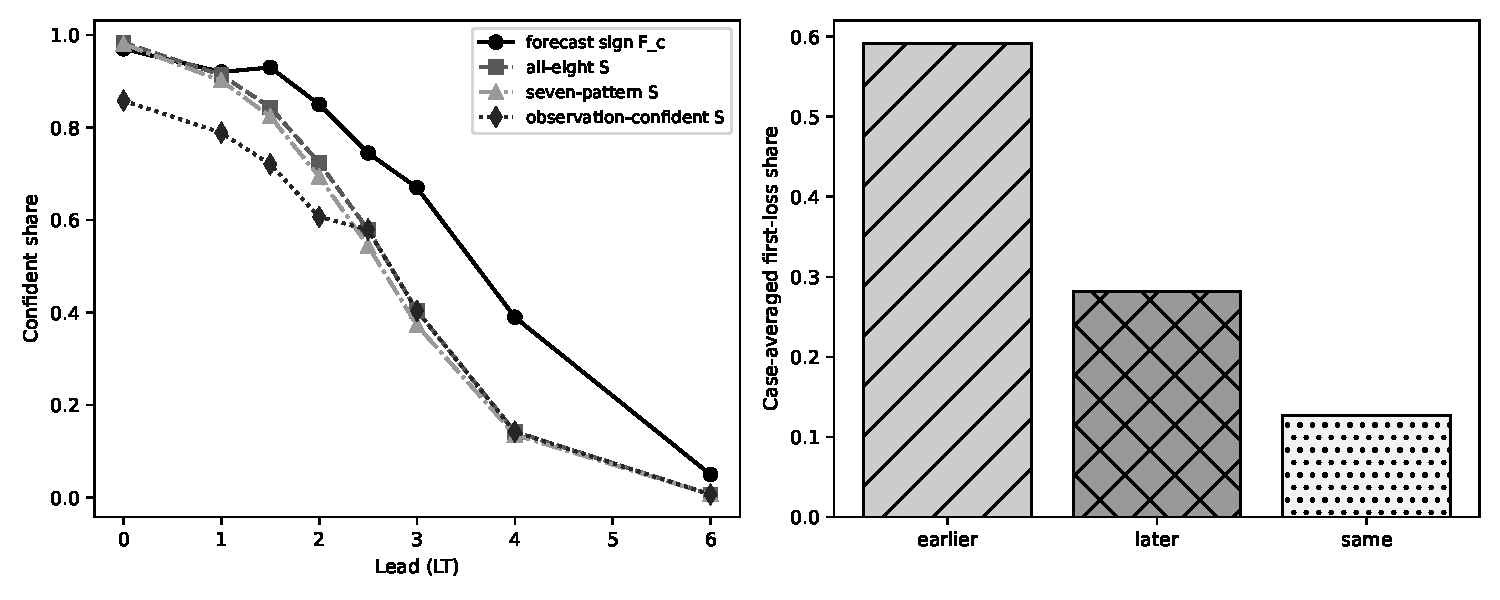
\includegraphics[width=\linewidth]{../figures/F15_overview_paper.pdf}
\caption{The two horizons, confirmation panel. Left: share of questions answered confidently against lead, for the forecast sign $F_c$ (solid, circles), all eight intervention signs (dashed, squares), the seven zero-mean patterns' signs (dash-dot, triangles) and observation-confident intervention signs (dotted, diamonds). Right: for the 1332 eligible actions, case-averaged shares whose intervention-sign confidence is lost earlier than, later than, or at the same lead as forecast-sign confidence (hatched bars; pre-registered reading).}
\label{fig:overview}
\end{figure}

\begin{figure}[t]
\centering
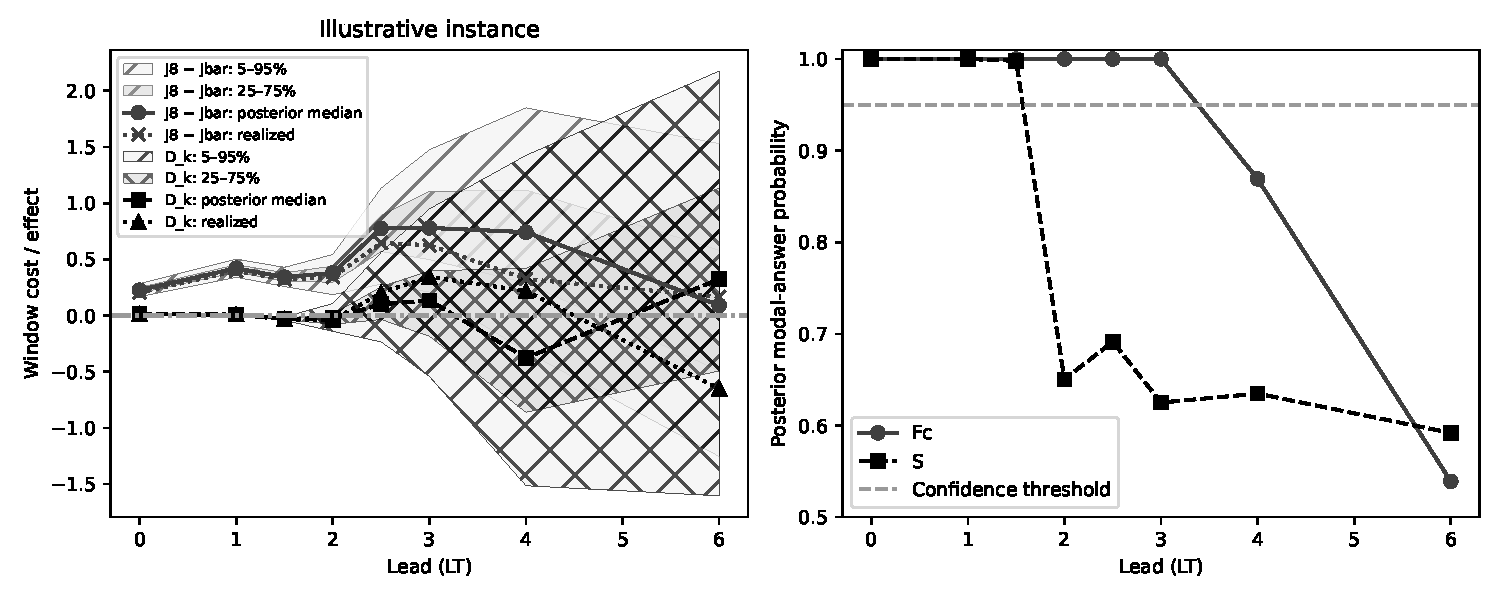
\includegraphics[width=\linewidth]{../figures/F16_instance_paper.pdf}
\caption{Post hoc, illustrative: one instance (case 3, $m = 2$ cosine pattern), selected by the rule in the text. Left: posterior 5--95\% and 25--75\% bands (shaded or hatched, as in the legend) and medians of the forecast anomaly $J_8 - \Jbar$ (circles) and the intervention effect $D_k$ (squares) against lead, with the realized values (crosses, triangles). Right: posterior probability of the modal answer for the forecast sign (solid, circles) and the intervention sign (dashed, squares), with the 0.95 threshold (dashed line).}
\label{fig:instance}
\end{figure}

\subsection{Confident answers are right}
Table~\ref{tab:calibration} gives the case-averaged accuracy of observation-confident intervention-sign answers at every lead. Accuracy passes the 0.90 criterion at every lead with enough answers to evaluate (up to 4~LT); at 6~LT only 11 such answers remain. Confident forecast-sign answers pass their own criterion (at least 30 confident instances and an exact one-sided 95\% lower bound of at least 0.90) at every lead where it can be evaluated. Over the reported questions (intervention and forecast signs at every lead, pairwise and best-action questions at 2 and 3~LT), the 15,202 confident answers are right 99.6\% of the time. Post hoc, answers below the confidence threshold are right about as often as their probability says (Figure~\ref{fig:emulators}, left), and the case-mean of modal probability minus correctness over the seven zero-mean patterns' intervention signs at 2~LT is $-0.002$ (99\% interval $[-0.064, 0.060]$), so mean calibration is not rejected. As supporting diagnostics of the sampler rather than evidence for the result, the true state and forcing lie inside the nominal 95\% likelihood-ratio region, $\Delta\chi^2 \le \chi^2_{0.95}(41)$, in 189 of 200 instances (94.5\%; Wilson 95\% interval $[90.4\%, 96.9\%]$), the posterior rank of the true forcing is consistent with uniform (Kolmogorov--Smirnov $p = 0.99$), and one instance in 200 is flagged by the goodness-of-fit test, against about 1\% expected.

\begin{table}[t]
\centering
\small
\caption{Accuracy of confident answers on the confirmation panel. $S$: case-averaged accuracy of observation-confident intervention-sign answers, with its one-sided 95\% betting lower bound, the number of such answers and of cases contributing. $F_c$: accuracy of confident forecast-sign answers (one per case) with its one-sided 95\% Clopper--Pearson lower bound.}
\label{tab:calibration}
\begin{tabular}{lccccc}
\toprule
Lead (LT) & $S$ accuracy & lower bound & answers & cases & $F_c$ accuracy [lower bound] \\
\midrule
0   & 1.000 & 0.983 & 1373 & 200 & 1.000 [0.985] \\
1   & 0.998 & 0.981 & 1262 & 199 & 1.000 [0.984] \\
1.5 & 0.999 & 0.982 & 1153 & 199 & 0.995 [0.975] \\
2   & 0.995 & 0.977 & 971  & 195 & 1.000 [0.983] \\
2.5 & 0.994 & 0.976 & 927  & 194 & 0.987 [0.958] \\
3   & 0.983 & 0.954 & 646  & 176 & 0.993 [0.965] \\
4   & 0.990 & 0.952 & 228  & 97  & 0.974 [0.921] \\
6   & \multicolumn{5}{c}{too few answers to evaluate (11 answers in 8 cases)} \\
\bottomrule
\end{tabular}
\end{table}

\subsection{Which is lost first}
\label{sec:order}
The pre-registered paired reading asks, within each instance, which confidence is lost first. An action is eligible if its sign is observation-confident and the forecast sign is confident at lead 0, which excludes the uniform decrease. For each eligible action we record the first tested lead at which each answer is no longer confident, and average, within each instance and then over instances, the indicator that the intervention sign is lost later minus the indicator that it is lost earlier. On 1332 eligible actions in 194 instances, intervention-sign confidence is lost before forecast-sign confidence for 59.1\% of an instance's eligible actions, after it for 28.2\% and at the same lead for 12.7\%. The difference, later minus earlier, is $-0.309$ (99\% interval $[-0.494, -0.128]$), which meets the pre-specified criterion. On the development panel it was $-0.210$ ($[-0.384, -0.016]$).

\paragraph{Robustness (post hoc).} Pooling pairs instead of averaging within instances gives the same shares (59.2\%, 28.1\% and 12.8\%). Counts are 788 earlier, 374 later and 170 at the same lead. An answer that stays confident at every tested lead through 6~LT is counted as lost after 6~LT; this applies to the intervention sign for 2 pairs, to the forecast sign for 35 and to both for none. Each of the seven patterns shows the same ordering, with earlier loss for between 54.7\% and 61.1\% of eligible actions and later loss for between 25.4\% and 31.1\%. Table~\ref{tab:sweep} repeats the reading at confidence thresholds of 0.90 and 0.99, applied to the posterior and to climatology alike: the difference stays between $-0.29$ and $-0.31$ with every 99\% interval below zero. The first loss is not always permanent: confidence returns at a later tested lead for 29.3\% of eligible intervention-sign pairs and 31.9\% of forecast-sign pairs. Comparing the last confident lead instead of the first non-confident one strengthens the ordering ($-0.487$, $[-0.610, -0.322]$).

Each probability is a share of correlated Markov chain draws. Over the eligible pairs at 2~LT, the bulk effective sample size of the intervention-sign modal-answer indicator has median 1695 (interquartile range 512 to 2000), and 5.6\% of these probabilities at 2~LT and 7.8\% at 3~LT lie within two Monte Carlo standard errors of 0.95. Setting every such borderline answer, at every lead, in the direction least favourable to the result (borderline intervention signs confident, borderline forecast signs not) gives $-0.249$ ($[-0.442, -0.078]$); the opposite assignment gives $-0.367$ ($[-0.548, -0.190]$).

\begin{table}[t]
\centering
\small
\caption{Post hoc threshold sweep, confirmation panel. The confidence threshold applies to the posterior and to climatology. First loss: paired difference, later minus earlier, on the pairs eligible at that threshold (1358, 1332 and 1287). Last confident: the same with the last confident lead. Seven minus $F_c$: same-lead difference between the seven-pattern confident $S$ share and the confident $F_c$ share. Accuracy: case-averaged accuracy of observation-confident $S$ answers at 2~LT with its one-sided 95\% lower bound. Brackets are 99\% betting intervals unless stated.}
\label{tab:sweep}
\begin{tabular}{lccc}
\toprule
Reading & threshold 0.90 & 0.95 & 0.99 \\
\midrule
First loss & $-0.290$ [$-0.470$, $-0.118$] & $-0.309$ [$-0.494$, $-0.128$] & $-0.297$ [$-0.490$, $-0.128$] \\
Last confident & $-0.441$ [$-0.568$, $-0.268$] & $-0.487$ [$-0.610$, $-0.322$] & $-0.462$ [$-0.614$, $-0.318$] \\
Seven minus $F_c$, 2~LT & $-0.128$ [$-0.234$, $-0.022$] & $-0.156$ [$-0.270$, $-0.046$] & $-0.188$ [$-0.318$, $-0.074$] \\
Seven minus $F_c$, 3~LT & $-0.231$ [$-0.348$, $-0.102$] & $-0.298$ [$-0.420$, $-0.182$] & $-0.251$ [$-0.384$, $-0.132$] \\
Accuracy, 2~LT & 0.987 [0.968] & 0.995 [0.977] & 1.000 [0.982] \\
\bottomrule
\end{tabular}
\end{table}

\subsection{The intervention sign is confident less often than the forecast sign}
\label{sec:samelead}
Figure~\ref{fig:overview} (left) and Appendix Figure~\ref{fig:confidence} show the confident share of each question type against lead. Immediately after the observation window 98.3\% of intervention-sign questions and 97.0\% of forecast signs are confident at lead 0, and 91.4\% against 92.0\% at 1~LT. The shares then separate: 84.4\% against 93.0\% at 1.5~LT, 72.4\% against 85.0\% at 2~LT, 40.4\% against 67.0\% at 3~LT, and 14.25\% against 39.0\% at 4~LT. The panel forecast horizon defined in Section~\ref{sec:setup} is therefore 3~LT. Of the confident intervention-sign answers at 2~LT, 16.1\% are given by climatology, all of them for the uniform decrease. The pre-specified same-lead difference between the observation-confident $S$ share and the confident $F_c$ share is $-0.243$ at 2~LT (99\% interval $[-0.352, -0.136]$) and $-0.266$ at 3~LT ($[-0.388, -0.152]$); both meet the criterion. The development panel gave $-0.221$ ($[-0.322, -0.106]$) at 2~LT. Pairwise orderings are confident for 74.0\% of pairs at 2~LT and 43.3\% at 3~LT, and the best action is confident for 65.0\% and 20.5\% of instances.

The pre-specified comparison removes the uniform decrease's climate-given answers from the intervention side only, which widens the gap at 2~LT. Post hoc, Table~\ref{tab:seven} compares like with like. Over all eight patterns, the all-confident $S$ share minus the confident $F_c$ share is $-0.126$ at 2~LT (99\% interval $[-0.234, -0.018]$) and $-0.266$ at 3~LT. Restricted to the seven patterns whose sign climatology never gives, it is $-0.156$ ($[-0.270, -0.046]$) and $-0.298$ ($[-0.420, -0.182]$). Each of the seven is confident less often than the forecast sign at both leads (Figure~\ref{fig:patterns}): between 64.0\% and 76.0\% against 85.0\% at 2~LT, and between 26.5\% and 46.0\% against 67.0\% at 3~LT. At a threshold of 0.90 the all-eight difference at 2~LT is $-0.104$ ($[-0.204, -0.002]$), the narrowest margin in the sweep.

Post hoc, for context, the posterior-mean forecast of the unforced state remains accurate by conventional measures over these leads. Its window-mean anomaly correlation with the true state is 0.983 at 2~LT, 0.928 at 3~LT and 0.815 at 4~LT, and its window-mean RMS error is 0.120, 0.268 and 0.440 of $\sigma$. At 3~LT, with an anomaly correlation of 0.93, the intervention sign is confident for 37.2\% of the seven patterns' questions.

\begin{table}[t]
\centering
\small
\caption{Post hoc: confident shares by lead, confirmation panel. Seven: intervention-sign questions for the seven patterns climatology does not answer. All: all eight patterns. The difference is the case-level mean of the seven-pattern confident share minus the confident-$F_c$ indicator, with its 99\% betting interval.}
\label{tab:seven}
\begin{tabular}{lcccc}
\toprule
Lead (LT) & seven $S$ & all $S$ & $F_c$ & seven minus $F_c$ [99\%] \\
\midrule
0   & 98.1\% & 98.3\% & 97.0\% & $+0.011$ [$-0.056$, $0.080$] \\
1   & 90.1\% & 91.4\% & 92.0\% & $-0.019$ [$-0.098$, $0.066$] \\
1.5 & 82.4\% & 84.4\% & 93.0\% & $-0.106$ [$-0.192$, $-0.016$] \\
2   & 69.4\% & 72.4\% & 85.0\% & $-0.156$ [$-0.270$, $-0.046$] \\
2.5 & 54.4\% & 57.9\% & 74.5\% & $-0.201$ [$-0.320$, $-0.072$] \\
3   & 37.2\% & 40.4\% & 67.0\% & $-0.298$ [$-0.420$, $-0.182$] \\
4   & 13.6\% & 14.25\% & 39.0\% & $-0.254$ [$-0.354$, $-0.128$] \\
6   & 0.7\% & 0.7\% & 5.0\% & $-0.043$ [$-0.112$, $0.026$] \\
\bottomrule
\end{tabular}
\end{table}


\begin{figure}[t]
\centering
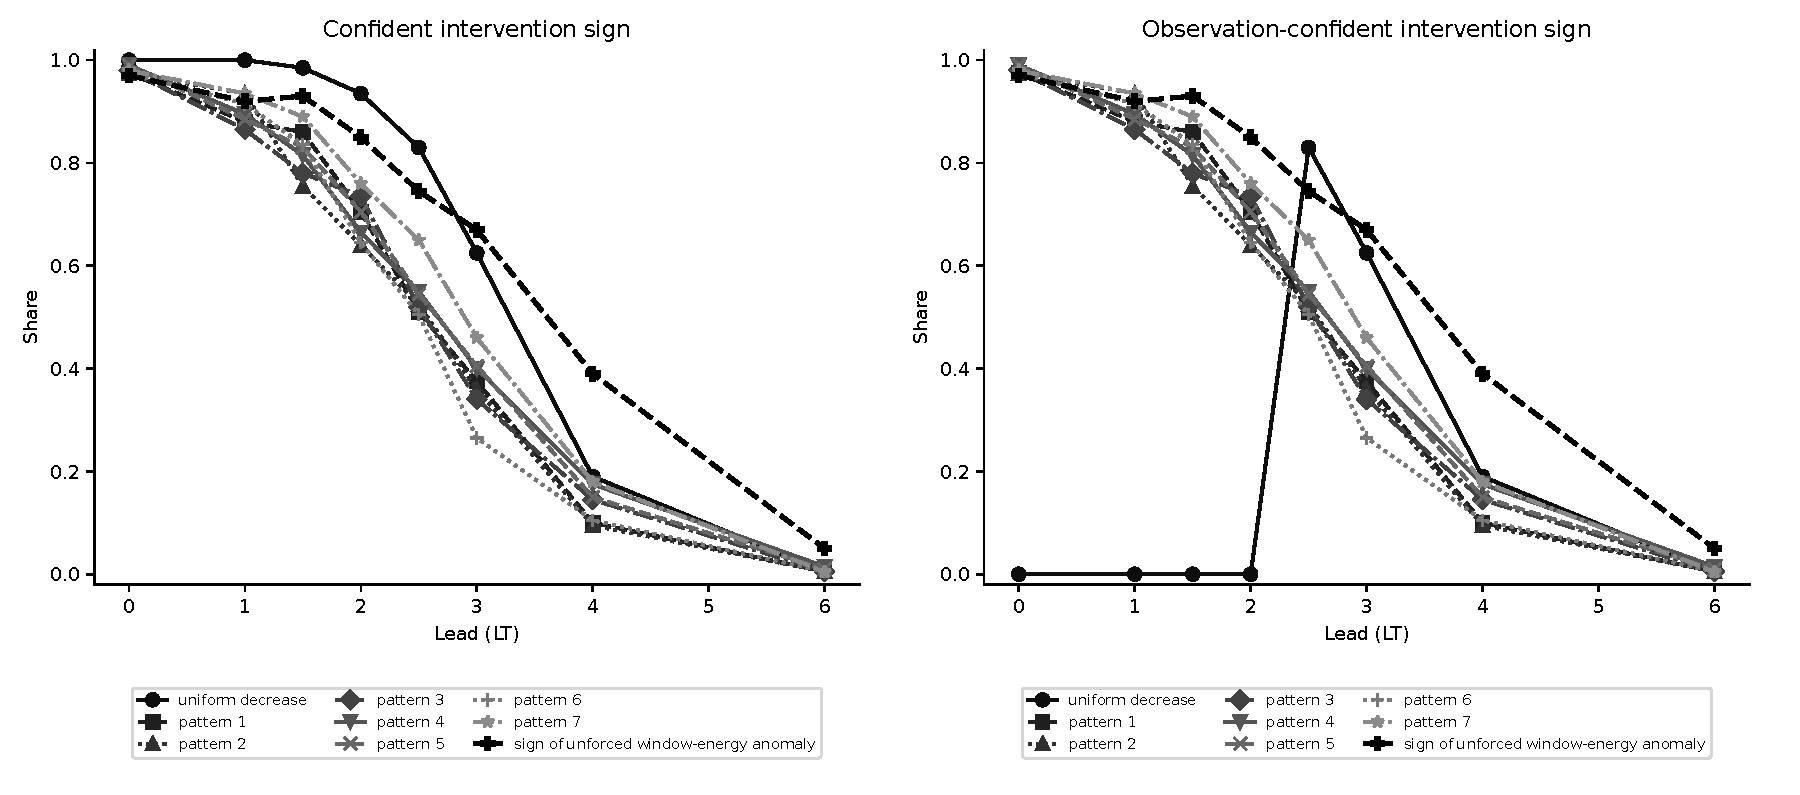
\includegraphics[width=0.55\linewidth,trim=0 0 444 0,clip]{../figures/F7_patterns.pdf}
\caption{Post hoc: confident intervention-sign share for each pattern against lead, with the forecast sign (dashed, plus markers) as reference. Each pattern has its own combination of line style and marker. The uniform decrease (solid circles) is the one pattern whose sign climatology gives up to 2~LT.}
\label{fig:patterns}
\end{figure}

\subsection{A second observable and the time step (post hoc)}
\label{sec:block}
For a block of sites the advection term no longer conserves energy: the block's energy changes also through transport across its boundaries, so the global budget does not carry over. We repeated the comparison for the energy of the 10-site block $i = 0,\dots,9$, specified before the block-observable results were read, with its own climatological mean and realized answers. The single-site pattern's large change (at site 0) lies inside this block. The result is the same (Figure~\ref{fig:block}). Block intervention signs are confident for 70.25\% of questions against 83.0\% for the block forecast sign at 2~LT, and 41.6\% against 64.0\% at 3~LT. The seven-pattern differences are $-0.141$ ($[-0.242, -0.010]$) and $-0.235$ ($[-0.368, -0.168]$), and the paired difference is $-0.254$ ($[-0.444, -0.114]$), with earlier loss for 54.9\% and later loss for 29.5\% of eligible actions. Confident block intervention-sign answers are right 99.6\% of the time at 2~LT (case-averaged; one-sided 95\% lower bound 97.7\%).

The pre-panel step-size check covered leads up to 3~LT, while the paired reading uses leads through 6~LT, whose window ends 7~LT after the action. We therefore re-integrated every saved draw, the truth and the climatological ensemble at $\Delta t = 0.005$ through 7~LT. No intervention-sign or forecast-sign confidence classification changes at any lead, Table~\ref{tab:calibration} is unchanged, and the paired difference is unchanged ($-0.309$, $[-0.494, -0.128]$). Four pairwise classifications change, one at 3~LT and three at 4~LT. The share of draw-level intervention-sign answers that change is at most 0.0011, at 6~LT. Realized intervention-sign answers change for 3 questions, all at 6~LT, and no realized forecast-sign answer changes. (The pre-panel check used separate check cases.)

\begin{figure}[t]
\centering
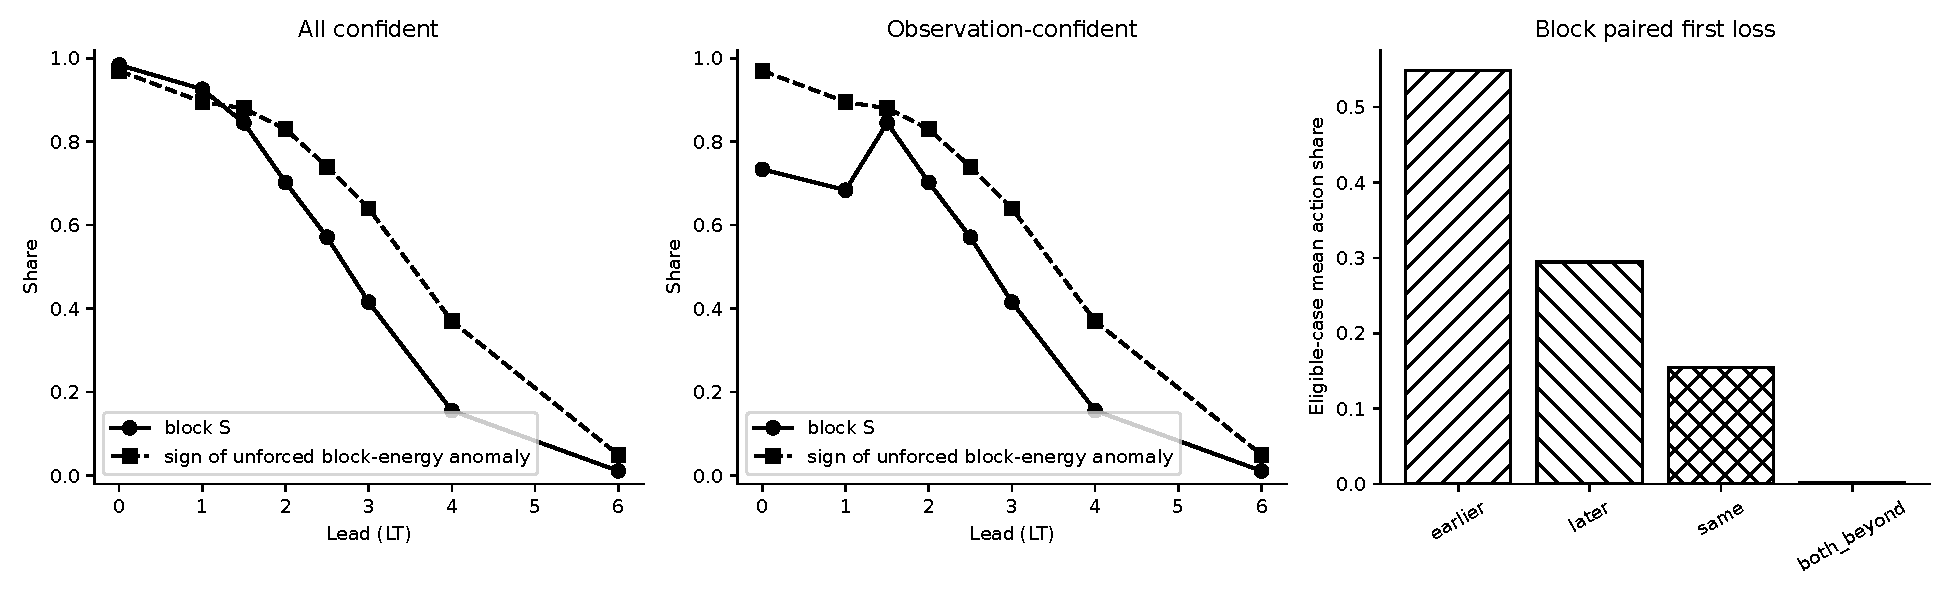
\includegraphics[width=\linewidth]{../figures/F9_block.pdf}
\caption{Post hoc: energy of sites 0--9, confirmation panel. Left and centre: all-confident and observation-confident block intervention-sign shares (solid circles) against the block forecast sign (dashed squares). Right: case-averaged paired first-loss categories (hatched bars).}
\label{fig:block}
\end{figure}

%======================================================================
\section{Why shared uncertainty does not settle the sign}
\label{sec:mechanism}

\subsection{Correlation without resolution}
\label{sec:readout}
For each instance, action and lead we compute the posterior correlation $\rho_k$ between $J_k$ and $J_8$, the share of the summed variance left in the difference, $c_k = \operatorname{Var}(D_k)/[\operatorname{Var}(J_k) + \operatorname{Var}(J_8)] = 1 - 2\operatorname{Cov}(J_k, J_8)/[\operatorname{Var}(J_k) + \operatorname{Var}(J_8)]$, and two signal-to-noise ratios, $z_D = |\mathbb E D_k| / \operatorname{sd}(D_k)$ for the intervention and $z_F = |\mathbb E J_8 - \Jbar| / \operatorname{sd}(J_8)$ for the forecast anomaly. Table~\ref{tab:mechanism} and Figure~\ref{fig:mechanism} give their medians over the panel. Just after the window the factual and counterfactual window energies are almost perfectly correlated (median $\rho = 0.99999$, median $c \approx 10^{-5}$), and the intervention's effect is resolved far more sharply than the forecast anomaly: the median $z_D$ is 3.6 times the median $z_F$. The correlation then decays only slightly, to 0.975 at 2~LT, but $c$ grows by more than three orders of magnitude, to 0.031, and the median $z_D$ falls below the median $z_F$ from 1.5~LT, to 0.61 times it at 2~LT. Confidence tracks $c$: among case--action--lead triples with $c < 0.1$, 86.9\% of intervention signs are confident, against 51.2\% for $0.1 \le c < 0.25$, 28.9\% for $0.25 \le c < 0.5$ and 9.3\% for $0.5 \le c < 1$ (descriptive bins pooling instances, actions and leads). The intervention's footprint on the state does not shrink: from about 1~LT on, the posterior-mean RMS separation between factual and counterfactual trajectories stays between 1.43 and 1.54 times the posterior RMS spread of the factual state (window medians). Why does a correlation of 0.975 leave the sign so often unresolved?

\begin{table}[t]
\centering
\small
\caption{Mechanism readout, confirmation panel: panel medians of the posterior correlation $\rho$ between factual and counterfactual window energies, the variance share left in their difference $c$, and the signal-to-noise ratios of the intervention effect ($z_D$) and the forecast anomaly ($z_F$). The last column is the ratio of the two medians. These are descriptive.}
\label{tab:mechanism}
\begin{tabular}{lccccc}
\toprule
Lead (LT) & median $\rho$ & median $c$ & median $z_D$ & median $z_F$ & ratio \\
\midrule
0   & 1.000 & $1.1\times10^{-5}$ & 62.0 & 17.3 & 3.58 \\
1   & 0.999 & $8.2\times10^{-4}$ & 13.4 & 10.5 & 1.27 \\
1.5 & 0.995 & 0.006 & 7.25 & 8.51 & 0.85 \\
2   & 0.975 & 0.031 & 3.68 & 6.05 & 0.61 \\
2.5 & 0.913 & 0.102 & 2.07 & 3.77 & 0.55 \\
3   & 0.778 & 0.244 & 1.21 & 2.28 & 0.53 \\
4   & 0.348 & 0.669 & 0.59 & 1.24 & 0.48 \\
6   & 0.064 & 0.937 & 0.25 & 0.34 & 0.74 \\
\bottomrule
\end{tabular}
\end{table}

\begin{figure}[t]
\centering
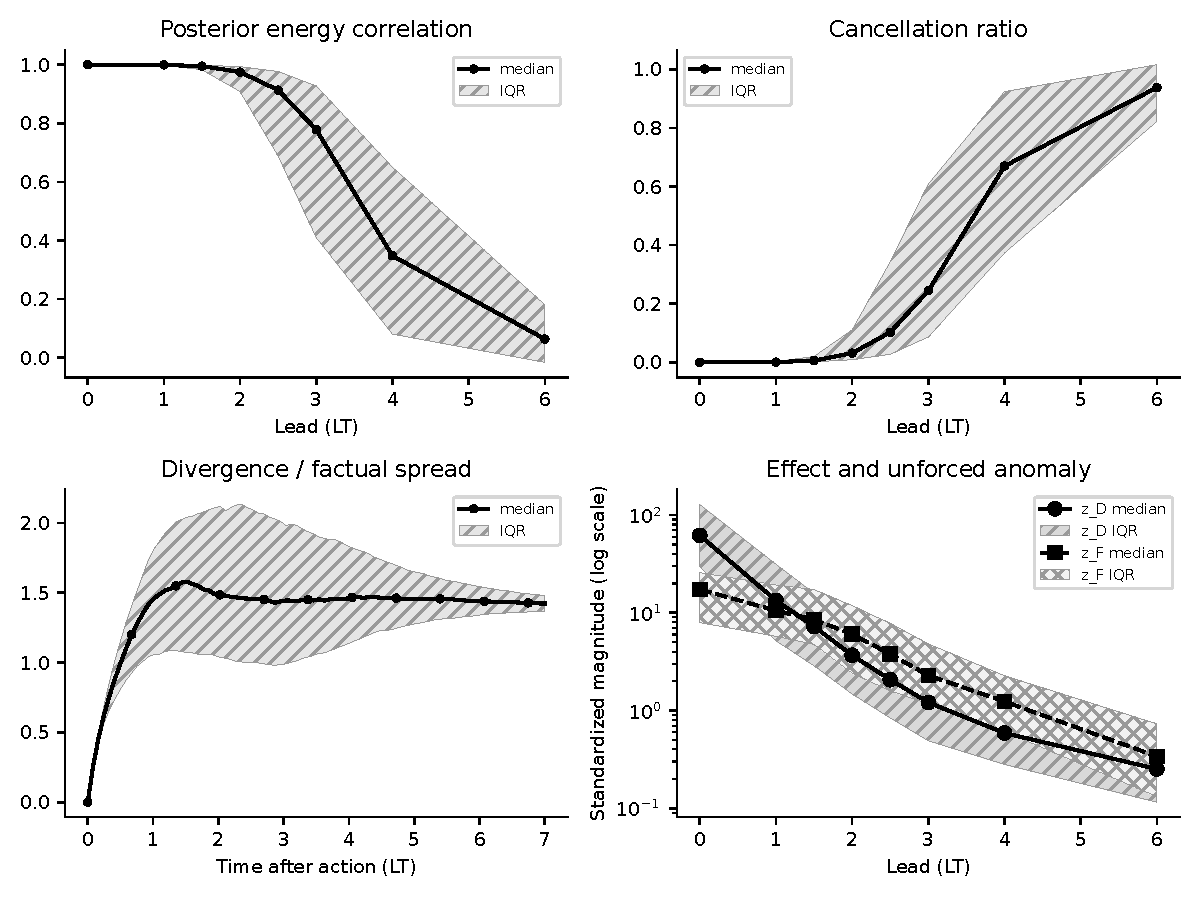
\includegraphics[width=0.92\linewidth]{../figures/F3_mechanism.pdf}
\caption{Mechanism, confirmation panel; medians with interquartile bands. Top: posterior correlation between factual and counterfactual window energies, and the share of their summed variance left in the difference. Bottom left: posterior-mean RMS separation between factual and counterfactual states divided by the posterior RMS spread of the factual state, against time after the action. Bottom right: signal-to-noise ratio of the intervention effect ($z_D$, solid circles, hatched band) and of the forecast anomaly ($z_F$, dashed squares, cross-hatched band), log scale.}
\label{fig:mechanism}
\end{figure}

\subsection{A small-amplitude limit}
\label{sec:prop}
Write $D_k(a)$ for the effect of action $k$ at amplitude $a$ for a given draw and lead, and $G_k = \partial D_k/\partial a$ at $a = 0$ for its tangent (linear) response. The Runge--Kutta map at a fixed step is polynomial in the state and in $a$, and the time-zero state does not depend on $a$, so $D_k(a)$ is a polynomial, hence smooth, in $a$ for every draw, with $D_k(0) = 0$. Probabilities and moments are under the posterior given the observations $Y$. The statement applies equally to the empirical distribution of the saved draws: there the moment conditions hold automatically, and if no draw has $G_k = 0$, the share of draws with $D_k(a) < 0$ equals the share with $G_k < 0$ for all sufficiently small $a > 0$.

\begin{proposition}
\label{prop:small}
Fix a lead and an action. Suppose that $J_8$ and $G_k$ have finite, non-zero posterior variance, that $\sup_{|b| \le a_0} |\partial^2 D_k(b)/\partial b^2|$ has a finite second moment for some $a_0 > 0$, and that $P(G_k = 0 \mid Y) = 0$. Then as $a \to 0^+$:
\begin{enumerate}
\item[(i)] $c_k(a) = a^2 \operatorname{Var}(G_k) / [2 \operatorname{Var}(J_8)] + O(a^3)$, and $\rho_k(a) \to 1$;
\item[(ii)] $z_D(a) \to |\mathbb E\, G_k| / \operatorname{sd}(G_k)$;
\item[(iii)] $P(D_k(a) < 0 \mid Y) \to P(G_k < 0 \mid Y)$.
\end{enumerate}
The analogous limits hold under the climatological ensemble.
\end{proposition}

\begin{proof}
Taylor's theorem gives $D_k(a) = a G_k + a^2 R(a)$ with $|R(a)| \le \frac12 \sup_{|b| \le a_0} |\partial^2 D_k/\partial b^2|$ for $|a| \le a_0$, so $\mathbb E R(a)^2$ is bounded. Hence $\operatorname{Var} D_k(a) = a^2 \operatorname{Var} G_k + O(a^3)$ and $\operatorname{Cov}(J_8, D_k(a)) = O(a)$, so $\operatorname{Var} J_k = \operatorname{Var} J_8 + O(a)$. Then (i) follows from $c_k = \operatorname{Var} D_k / (\operatorname{Var} J_k + \operatorname{Var} J_8)$ and $\rho_k = [\operatorname{Var} J_8 + \operatorname{Cov}(J_8, D_k)] / (\operatorname{Var} J_8 \operatorname{Var} J_k)^{1/2}$, and (ii) from dividing $\mathbb E D_k$ and $\operatorname{sd} D_k$ by $a$. For (iii), $D_k(a)/a \to G_k$ for every draw, so $D_k(a)/a$ converges in distribution to $G_k$, and 0 is a continuity point because $P(G_k = 0 \mid Y) = 0$; for $a > 0$, $D_k(a) < 0$ exactly when $D_k(a)/a < 0$.
\end{proof}

The result is elementary, but it removes the apparent paradox. By (i), the correlation between factual and counterfactual futures tends to one at every lead as the intervention shrinks, whatever the sign's confidence; by (iii), that confidence tends to a limit set by the posterior distribution of $G_k$, and the classification as confident converges too unless that limit is exactly 0.95. A small $c$ says that the effect's spread is small relative to the marginal forecast spreads, which shrinking the intervention guarantees (and with it $\rho_k \to 1$, since $\rho_k \ge 1 - c_k$ whenever $c_k < 1$). It does not say whether the effect's mean is large relative to its own spread, which is what the sign's confidence depends on. In these results, at fixed amplitude, confidence falls as $c$ grows (Section~\ref{sec:readout}; an empirical association), but shrinking $a$ sends $c$ to zero without changing the limiting confidence. The intervention question is decided by $G_k$, the derivative of the window energy along $p_k$, and the forecast question by $J_8 - \Jbar$: two functionals of one posterior. The proposition imposes no order on the leads at which they stop being confident; that order is an empirical property of this system, observation design and question. To leading order in $a$, a larger intervention has a proportionally larger effect and the same sign confidence; the first correction can go either way. The climatological probabilities also converge, so at small amplitude which answers climatology gives does not depend on amplitude. Moreover, Lorenz-96 is equivariant under cyclic shifts of the sites and $G_k$ is linear in $p_k$, so under any shift-invariant climatological distribution the mean of $G_k$ is zero for every zero-mean pattern at every lead. A zero mean does not by itself make the two signs equally likely; post hoc, in the 4096-state climatological ensemble the largest departure of the mean of $G_k$ from zero, over the zero-mean patterns and leads, is 0.034 standard deviations, and the share of states with $G_k < 0$ lies between 0.454 and 0.510. For the uniform decrease the climatological share with $G_k < 0$ is 0.980 at 2~LT and 0.945 at 2.5~LT, in line with climatology giving its sign up to 2~LT.

\subsection{The tangent response reproduces the classifications (post hoc)}
\label{sec:tangent}
We computed $G_k$ for every saved draw, action and lead by a hand-coded forward-mode (tangent-linear) recursion through every Runge--Kutta stage. On 8 draws for every pattern and lead it agrees with JAX's automatic differentiation of the same map to $3.4\times10^{-10}$, and on 4 draws with centred finite differences to $2.4\times10^{-8}$ (scaled by $1 + |G_k|$) through 3~LT. We compared it with the finite effect re-forecast at $a = 0.04$ and $a = 0.64$, a quarter and four times the main amplitude (Figure~\ref{fig:tangent}). At $a = 0.04$, $D_k/a$ and $G_k$ have the same sign for 97.6\% of draws at 2~LT and 91.6\% at 3~LT, and classifying each question three ways (confident negative, not confident, confident positive) from the draws' $D_k$ and from their $G_k$ gives the same class for 96.7\% of questions at 2~LT (Cohen's $\kappa = 0.949$) and 96.1\% at 3~LT ($\kappa = 0.924$). The median $z_G$ is 3.51 at 2~LT, against 3.51 for $z_D$ at $a = 0.04$ and 3.68 at $a = 0.16$; at 3~LT it is 0.84, against 0.95 and 1.21. The main amplitude is thus close to the tangent limit at 2~LT and further from it at 3~LT. At $a = 0.64$ the limit no longer describes the answers: draw-level sign agreement is 77.1\% at 2~LT, and classification agreement is 63.3\% ($\kappa = 0.435$) at 2~LT and 56.3\% ($\kappa = 0.298$) at 3~LT.

\begin{figure}[t]
\centering
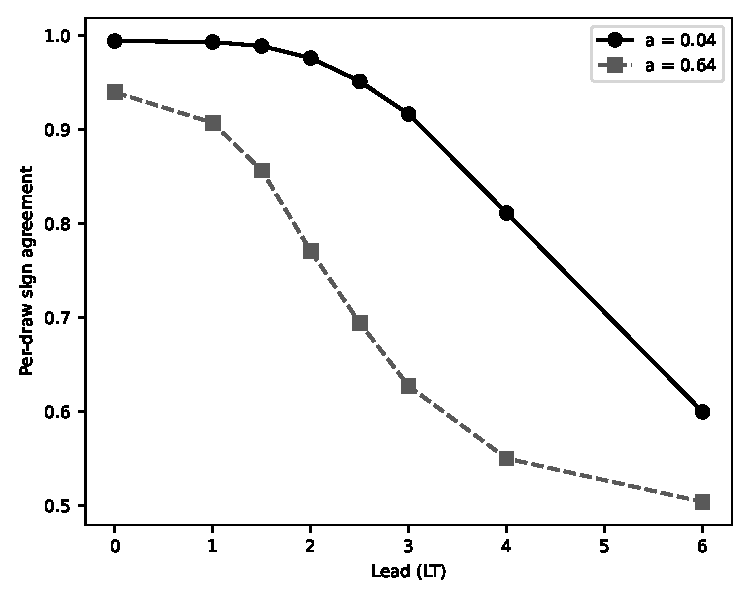
\includegraphics[width=0.5\linewidth]{../figures/F11_tangent_paper.pdf}
\caption{Post hoc, confirmation panel: share of draws for which the finite effect $D_k/a$ and the tangent response $G_k$ have the same sign, against lead, at $a = 0.04$ (solid circles) and $a = 0.64$ (dashed squares).}
\label{fig:tangent}
\end{figure}

\subsection{Two routes for the effect (post hoc)}
\label{sec:routes}
What, then, is $G_k$ made of? For Equation~\eqref{eq:l96} the advection term conserves energy, so $dE/dt = -2E + \frac{1}{N}\sum_i F_i x_i$. For the difference between the forced and unforced futures, $\Delta E = E_k - E_8$,
\begin{equation}
\frac{d\,\Delta E}{dt} = -2\,\Delta E + \underbrace{F\,(\bar x_k - \bar x_8)}_{\text{mean flow}} + \underbrace{\frac{a}{N}\sum_i p_{k,i}\, x_{k,i}}_{\text{direct injection}},
\qquad \bar x = \frac{1}{N}\sum_i x_i .
\label{eq:budget}
\end{equation}
Here $F$ is each draw's own forcing $F_s$. The second term is the work the unchanged forcing does on the change the intervention makes to the mean state; the third is the work the forcing change itself does. Since $\Delta E(0) = 0$, each term contributes to $D_k$ through the kernel $e^{-2(t-s)}$, with times in model units. Differentiating at $a = 0$ shows what each route depends on. The injection contributes $\frac1N \sum_i p_{k,i}\, x_{8,i}(s)$, a linear functional of the unforced trajectory: to first order it is determined by the unforced trajectory alone, so its uncertainty is forecast uncertainty. The mean flow contributes $F \bar\xi_k(s)$, where $\xi_k = \partial x_k/\partial a$ at $a = 0$ solves the tangent-linear equation $d\xi_k/dt = A(t)\,\xi_k + p_k$, $\xi_k(0) = 0$, with $A(t)$ the Jacobian of Equation~\eqref{eq:l96} along the unforced trajectory. This part depends on how the draw's flow responds to a perturbation, not only on where the flow goes. For a zero-mean pattern it exists only through the advection term, since $d\bar x/dt = R(2) - R(1) - \bar x + F$ with $R(m) = \frac1N\sum_i x_i x_{i+m}$ (the difference $R(2) - R(1)$ is unchanged if the mean is removed from each): the mean-flow route runs through the intervention's effect on the state's spatial covariance at lags one and two.

At the main amplitude, where the injection also includes the second-order term $\frac aN\sum_i p_{k,i}(x_{k,i} - x_{8,i})$, we recomputed every saved draw's factual and forced trajectories and integrated the two sources through Equation~\eqref{eq:budget}; they sum to $D_k$ up to an integration residual below $1.1\times10^{-5}$ (Figure~\ref{fig:budget}). The injection keeps a consistent sign across draws: at 2~LT its median $z$ is 10.2, against 3.3 for the mean-flow contribution, and at 3~LT 3.6 against 1.1. Within each case--action pair, the posterior variance of $D_k$ splits exactly into the variances of the two contributions and of the residual and their covariances (Figure~\ref{fig:variance}). For the seven zero-mean patterns the mean-flow share has median 0.948 at 1~LT, 0.995 at 2~LT and 0.998 at 3~LT, and the injection share 0.055, 0.0036 and 0.0007; for the uniform decrease the mean-flow share is 0.988 at 2~LT. Only at lead 0 does the injection dominate (median share 0.873 for the zero-mean patterns). Across case--action pairs, the share of draws disagreeing with the majority sign of the mean-flow contribution correlates with whether the intervention sign is confident at $-0.66$ at 2~LT and $-0.71$ at 3~LT, against $-0.10$ and $-0.13$ for the injection. These are descriptive: the draws disagree about the effect almost only through its mean-flow route, and no further causal attribution is inferred. A second exact split, $D_k = \frac{1}{N|W_T|}\sum_t x_8\cdot\delta x_k + \frac{1}{2N|W_T|}\sum_t \|\delta x_k\|^2$ with $\delta x_k = x_k - x_8$, shows how small the effect is relative to the state displacement: at 2~LT the projection term averages $-0.62$ and the displacement term $+0.58$ (averaged over instances and actions), so the effect is a small residual of two much larger terms, and a small relative error in either, such as an emulator's, can change its sign.

\begin{figure}[t]
\centering
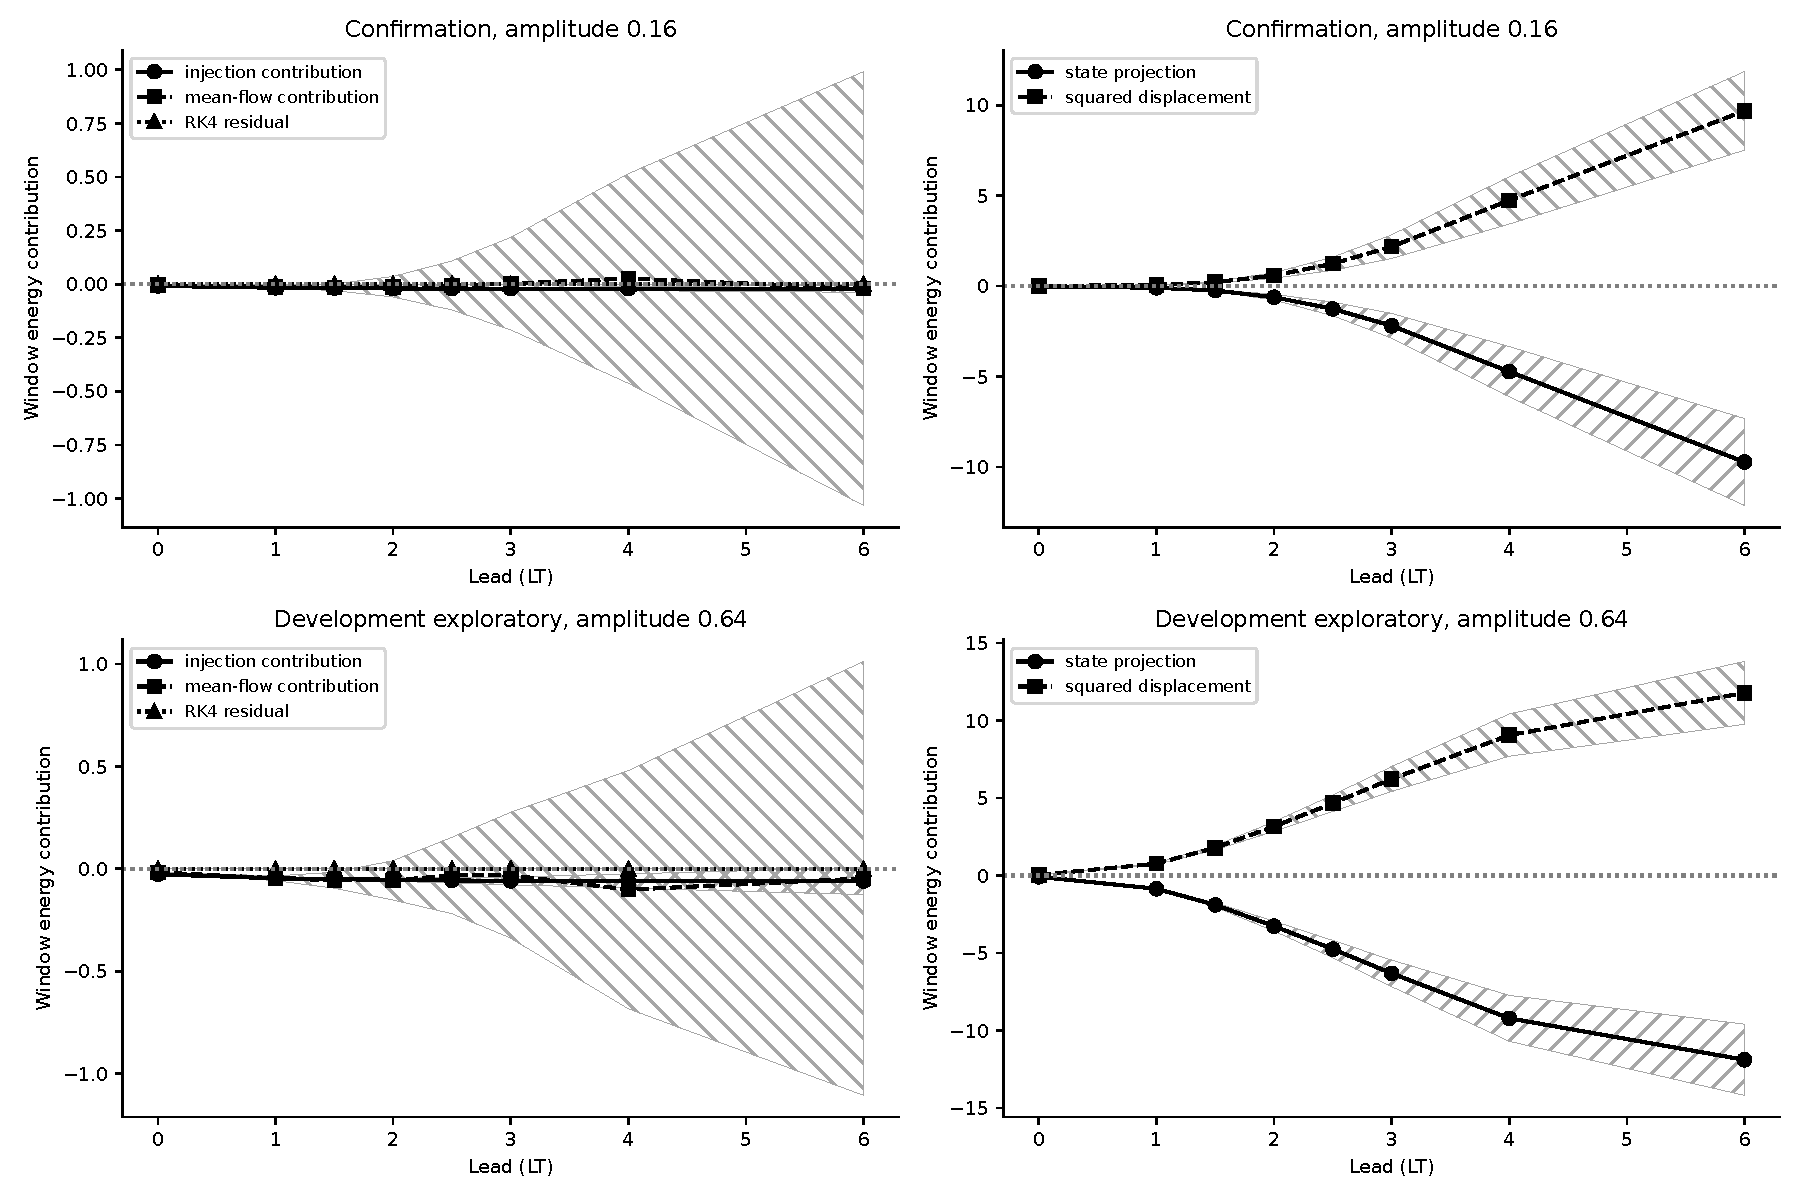
\includegraphics[width=0.92\linewidth,trim=0 288 0 0,clip]{../figures/F8_mechanism.pdf}
\caption{Post hoc: exact decompositions of the intervention's energy effect, confirmation panel, averaged over instances and actions; bands are $\pm$ the mean within-posterior standard deviation (descriptive). Left: contributions of the direct injection (solid circles), the mean flow (dashed squares) and the integration residual (dotted triangles) from Equation~\eqref{eq:budget}. Right: projection on the factual state (solid circles) and squared displacement (dashed squares).}
\label{fig:budget}
\end{figure}

\begin{figure}[t]
\centering
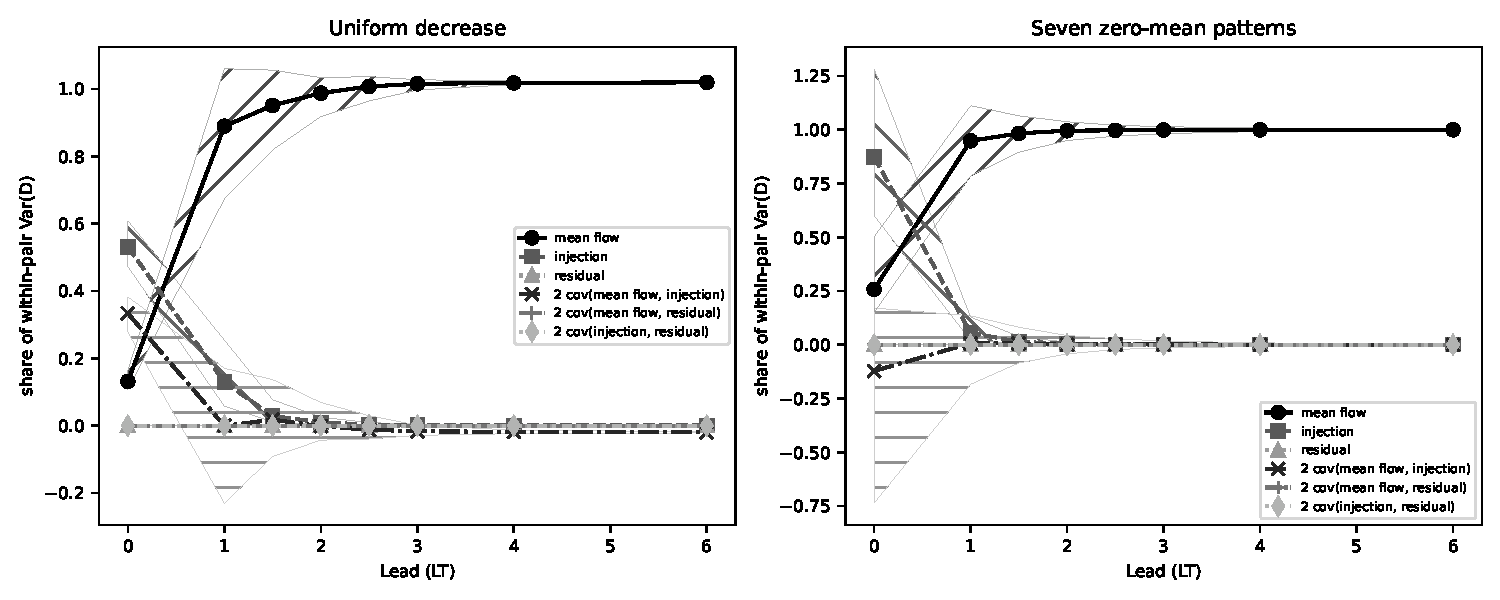
\includegraphics[width=\linewidth]{../figures/F12_variance_paper.pdf}
\caption{Post hoc: shares of the within-pair posterior variance of $D_k$, confirmation panel, median over case--action pairs with interquartile bands (hatched), for the uniform decrease (left) and the seven zero-mean patterns (right). The variances of the mean-flow, injection and residual contributions and twice their covariances; the six shares sum to one within each pair.}
\label{fig:variance}
\end{figure}

\subsection{Amplitude (post hoc)}
\label{sec:amplitude}
We re-forecast the saved confirmation draws at $a = 0.04$ and $a = 0.64$ (0.5\% and 8\% of the forcing in root-mean-square), re-ran the climatological ensemble at each amplitude, and scored the answers against the true state forced at that amplitude (Table~\ref{tab:amplitude}, Figure~\ref{fig:amplitude}). Confident answers stay right: observation-confident intervention-sign accuracy at 2~LT is 0.994 (lower bound 0.975) at $a = 0.04$ and 0.997 (0.980) at $a = 0.64$, and at 3~LT 0.984 (0.962) and 0.986 (0.957). Between $a = 0.04$ and $a = 0.16$ the confident share at 2~LT barely moves (71.1\% and 72.4\%), as expected if both amplitudes are near the tangent limit; at 3~LT it rises from 35.2\% to 40.4\%. At $a = 0.64$ the share rises, most at longer leads, and climatology gives some signs at 2.5 and 3~LT, which it does not at the smaller amplitudes; both are finite-amplitude effects. The paired ordering holds at every amplitude, with 99\% intervals below zero, and weakens as the amplitude grows: $-0.343$ at $a = 0.04$, $-0.309$ at 0.16 and $-0.208$ at 0.64. The same-lead seven-pattern difference at 2~LT includes zero at $a = 0.64$ ($-0.080$, $[-0.176, 0.010]$) but not at 3~LT ($-0.127$, $[-0.240, -0.014]$). Eligibility for the paired reading is re-evaluated at each amplitude (1320 and 1342 pairs). An exploratory sweep of five amplitudes on the development panel, without realized-outcome scoring at the changed amplitudes, gave the same pattern (paired difference from $-0.228$ at $a = 0.04$ to $-0.101$ at 0.64, with the intervals at 0.32 and 0.64 including zero).

\begin{table}[t]
\centering
\small
\caption{Post hoc: intervention amplitude, confirmation panel, with climatology re-run and realized answers recomputed at each amplitude. Confident intervention-sign shares (all eight patterns at 2~LT; the seven zero-mean patterns at 2 and 3~LT), the seven-pattern same-lead difference from $F_c$ (confident for 85.0\% at 2~LT and 67.0\% at 3~LT at every amplitude), and the paired first-loss difference. Brackets are 99\% betting intervals.}
\label{tab:amplitude}
\begin{tabular}{lccc}
\toprule
Amplitude $a$ & 0.04 & 0.16 & 0.64 \\
RMS change, \% of $F$ & 0.5 & 2 & 8 \\
\midrule
All $S$ confident, 2~LT & 71.1\% & 72.4\% & 79.75\% \\
Seven $S$ confident, 2~LT & 67.9\% & 69.4\% & 77.0\% \\
Seven $S$ confident, 3~LT & 31.9\% & 37.2\% & 54.3\% \\
Seven minus $F_c$, 2~LT & $-0.171$ [$-0.284$, $-0.056$] & $-0.156$ [$-0.270$, $-0.046$] & $-0.080$ [$-0.176$, $0.010$] \\
Seven minus $F_c$, 3~LT & $-0.351$ [$-0.480$, $-0.234$] & $-0.298$ [$-0.420$, $-0.182$] & $-0.127$ [$-0.240$, $-0.014$] \\
Paired first loss & $-0.343$ [$-0.534$, $-0.160$] & $-0.309$ [$-0.494$, $-0.128$] & $-0.208$ [$-0.370$, $-0.054$] \\
\bottomrule
\end{tabular}
\end{table}

\begin{figure}[t]
\centering
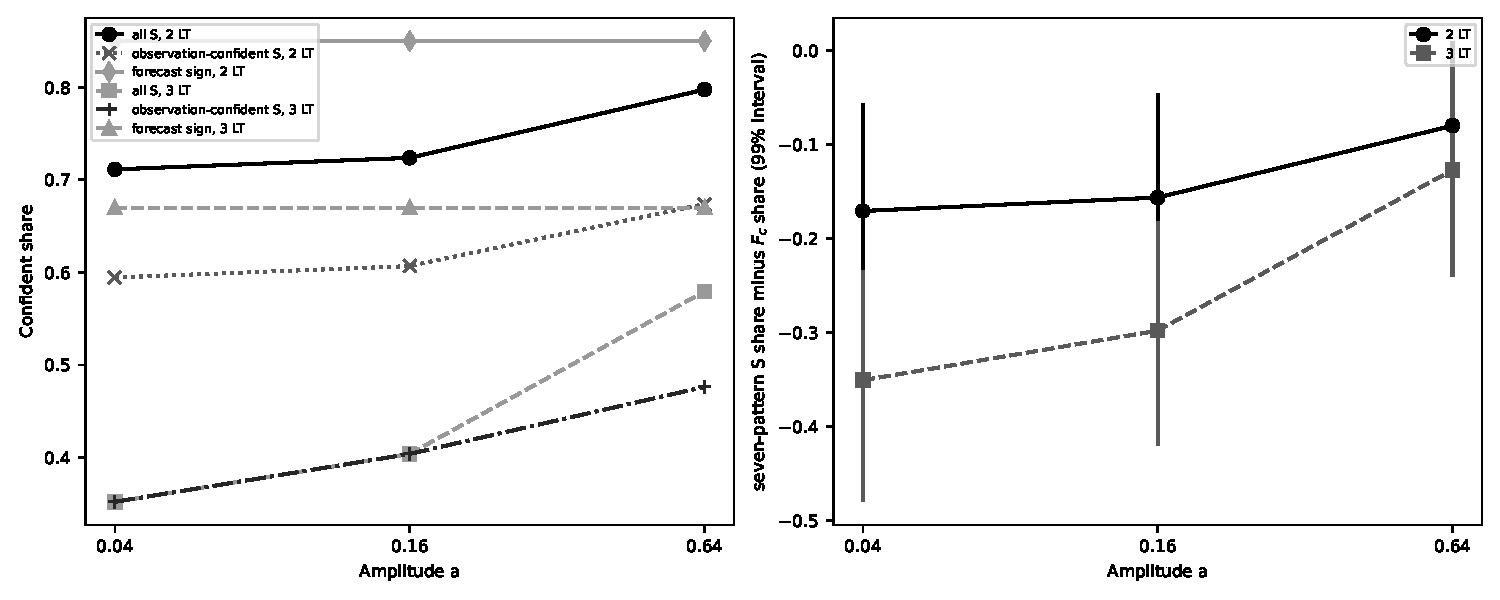
\includegraphics[width=\linewidth]{../figures/F14_amplitude_paper.pdf}
\caption{Post hoc: intervention amplitude, confirmation panel ($a = 0.04, 0.16, 0.64$, log scale). Left: all-confident (circles at 2~LT, squares at 3~LT) and observation-confident (crosses at 2~LT, plus signs at 3~LT) intervention-sign shares, with the forecast sign (diamonds at 2~LT, triangles at 3~LT) as reference. Right: seven-pattern same-lead difference from the forecast sign with 99\% betting intervals.}
\label{fig:amplitude}
\end{figure}

%======================================================================
\section{Forecast-matched models and decisions}
\label{sec:finding3}

\subsection{Learned emulators (post hoc)}
\label{sec:emulators}
Learned emulators of Lorenz-96 forecast it well from data \citep{chattopadhyay2020datadriven}. Do accurate forecasts give accurate intervention answers? To separate a learned model's dynamics from its representation of the uncertain state, we ran each emulator from every posterior draw's own noise-free 11-frame history, with the draw's action field and, for the forcing-conditioned emulators, the draw's own forcing, so that the uncertainty in the state (and, for those emulators, in the forcing) is the posterior's and the emulator supplies the dynamics. We scored each exactly as the posterior. The emulators share one architecture, a circular residual convolutional network of about $10^6$ parameters whose inputs are the 11 frames and the action field. CNN-20k, the emulator of the frozen protocol, was trained for 20,000 updates on 2048 trajectories at $F = 8$, with actions of random amplitude in $[-0.32, 0.32]$ on the eight patterns, observation noise added to its input histories, and a four-step autoregressive state loss; it has no forcing input. It is thus run on noise-free histories, unlike its training histories, and without each draw's forcing. CNN-F adds the forcing as an input channel and was trained, from scratch with the same loss and number of updates, on 4096 noise-free trajectories with $F$ uniform on $[6, 10]$ and the same distribution of actions (1.66 GPU-hours charged, including a discarded first run). Checkpoints were selected on held-out trajectories only.

Table~\ref{tab:emulators} and Figure~\ref{fig:emulators} give the results at 2~LT. CNN-20k forecasts the unforced state as accurately as the posterior (anomaly correlation 0.982 against 0.983) and is confident about as often (73.25\% of intervention signs against 72.4\%), but its confident intervention-sign answers are wrong 5.4\% of the time averaged over instances (5.5\% pooled), against 0.4\% (0.4\%) for the posterior; among answers that depend on the observations it is right 93.7\% of the time (lower bound 90.8\%) against 99.5\% (97.7\%). Its per-draw error in $D_k$ (RMS 0.087) is as large as its error in $J_8$ (0.085): its errors in the factual and counterfactual energies cancel only partly in the difference, whereas the posterior's spread in $D_k$ is a small fraction of its spread in $J_8$ (median $c = 0.031$). Its pooled error curve lies above the posterior's over their shared range of coverage (Figure~\ref{fig:emulators}, right), although its case-mean overconfidence ($+0.055$) does not reject mean calibration at the 1\% level. CNN-F is close to the posterior on every comparable reading in Table~\ref{tab:emulators}, with a confident error of 0.8\% (0.9\% pooled), and on the reliability curve; no equivalence test was specified, so this does not establish equivalence. It is a positive control: a learned model given the same uncertain states can pass this evaluation. Every emulator run on these draws reproduces the paired ordering, so the ordering does not depend on the exact integrator; because they share the posterior's draws, this does not test the sampler, which the development-panel ensemble smoother cross-checks (Section~\ref{sec:procedures}). CNN-F and CNN-20k differ in the forcing input, the training range of $F$, noise-free training histories and training-set size, and this comparison does not separate them. The paired ordering is the same for both emulators. At 3~LT the confident error is 4.9\% (bounds 2.2\% and 8.0\%) for CNN-20k, 1.1\% (0, 4.0\%) for CNN-F and 1.7\% (0, 4.6\%) for the posterior. Run instead as a 128-member ensemble of perturbed observation windows, as in the frozen protocol, CNN-20k is confident on 66.2\% of intervention signs at 2~LT and its confident observation-dependent answers are right 93.9\% of the time (lower and upper one-sided 95\% betting bounds 0.902 and 0.962). Both CNN-20k constructions meet the 0.90 accuracy criterion applied to the posterior, and neither meets the frozen protocol's condition for the word overconfident (accuracy below 0.85 with a one-sided 95\% betting upper bound below 0.90); they differ from the posterior in error rate, not by failing a criterion. These results concern these emulators and constructions, not learned world models in general.

\begin{table}[t]
\centering
\small
\caption{Post hoc: learned emulators run from each posterior draw's own history, confirmation panel, 2~LT. ACC and RMSE: window-mean anomaly correlation and RMS error ($/\sigma$) of the ensemble-mean unforced state against the truth. $D$ error: RMS per-draw error of $D_k$ against the same draw's physics. Confident $S$: share of intervention signs answered confidently. Error: case-averaged share of confident intervention-sign answers that are wrong, with one-sided 95\% betting bounds. Overconfidence: case-mean modal probability minus correctness over the seven zero-mean patterns' signs, with 99\% betting interval. Paired: first-loss difference on the posterior's 1332 eligible pairs, with 99\% betting interval.}
\label{tab:emulators}
\footnotesize
\setlength{\tabcolsep}{4pt}
\begin{tabular}{lcccccc}
\toprule
Model & ACC / RMSE & $D$ error & confident $S$ & error [bounds] & overconfidence [99\%] & paired [99\%] \\
\midrule
Posterior & 0.983 / 0.120 & --- & 72.4\% & 0.4\% [0, 2.2] & $-0.002$ [$-0.064$, $0.060$] & $-0.309$ [$-0.494$, $-0.128$] \\
CNN-20k & 0.982 / 0.123 & 0.087 & 73.25\% & 5.4\% [3.3, 7.8] & $+0.055$ [$-0.008$, $0.118$] & $-0.367$ [$-0.520$, $-0.208$] \\
CNN-F & 0.983 / 0.122 & 0.027 & 72.1\% & 0.8\% [0, 2.5] & $-0.001$ [$-0.064$, $0.060$] & $-0.292$ [$-0.486$, $-0.120$] \\
\bottomrule
\end{tabular}
\end{table}

\begin{figure}[t]
\centering
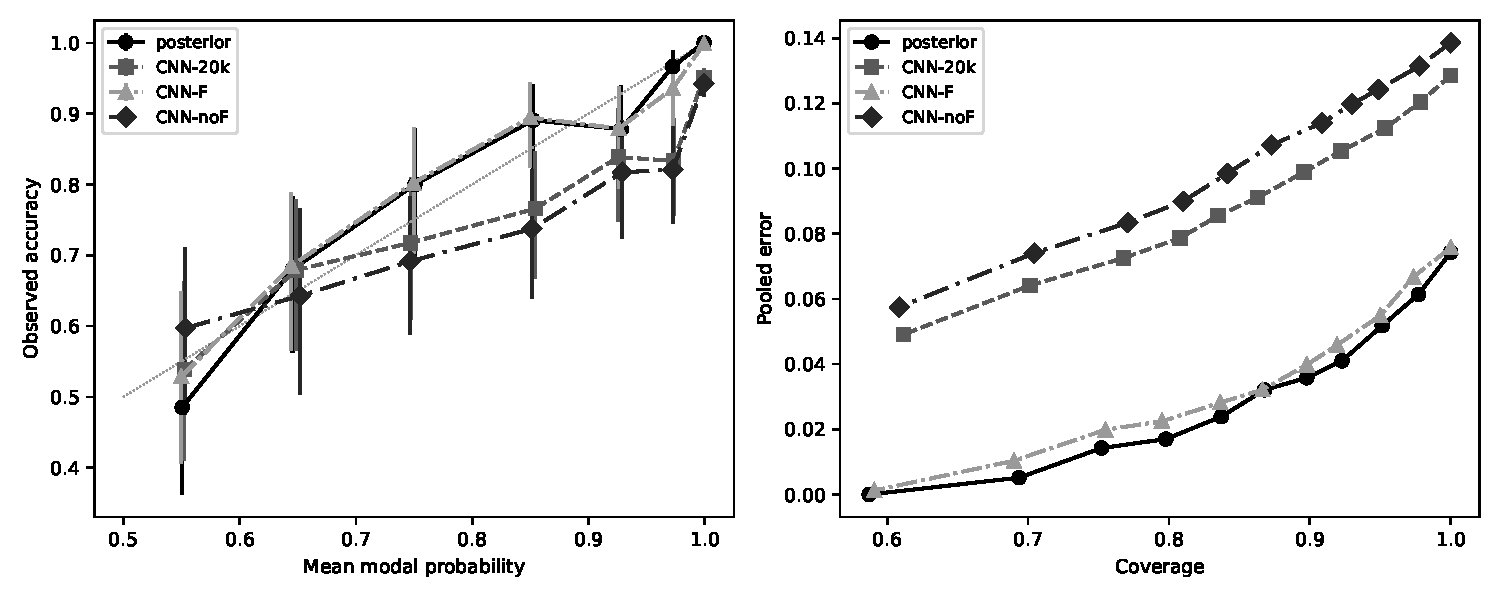
\includegraphics[width=\linewidth]{../figures/F13_main_paper.pdf}
\caption{Post hoc: the seven zero-mean patterns' 1400 intervention-sign questions at 2~LT, confirmation panel. Left: observed accuracy against mean modal probability in bins with edges 0.5, 0.6, 0.7, 0.8, 0.9, 0.95, 0.99 and 1; bars are pooled 95\% Clopper--Pearson intervals, descriptive because questions cluster within cases. Right: pooled error against the share of questions answered as the confidence threshold varies from 0.5 to 0.99. Posterior (solid, circles), CNN-20k (dashed, squares) and CNN-F (dash-dot, triangles); the dotted diagonal marks perfect reliability. Appendix Figure~\ref{fig:emulators_full} adds the other emulators.}
\label{fig:emulators}
\end{figure}

\subsection{Decisions (post hoc)}
\label{sec:decisions}
Does the distinction matter when choosing an action? Table~\ref{tab:decisions} compares five policies on the realized costs, each choosing among the nine options including no action. Policy E takes the option with the lowest posterior-mean window energy. Policy C takes E's choice only if the posterior is at least 95\% confident that it lowers the energy by more than a margin $\delta$ (a fraction of the climatological standard deviation of $D_k$), and otherwise does nothing. The baselines are doing nothing and always taking the uniform decrease, the one action whose sign climatology gives. A harm is a realized window energy above that of doing nothing.

Acting on the posterior mean gives the largest improvement and the lowest regret. Always decreasing the forcing is a strong baseline at 2~LT but not at 3~LT, where it harms 30 of 200 instances. Requiring confidence harmed none of the 200 instances at either lead (one-sided 95\% Clopper--Pearson upper bound on the harm rate 1.49\%), whereas E harmed one instance at 2~LT and nine at 3~LT; E's harms are rare but can be large (1.63 at 2~LT, more than five times E's mean improvement). The price is forgone gains: at 3~LT C acts in 70.5\% of instances and its regret is more than twice E's. Raising the margin to 0.1 of the climatological standard deviation leaves C unchanged at 2~LT and changes it little at 3~LT (acting 70.5\% to 66.5\%). These are results for these 200 instances. Losing confidence in many intervention signs therefore does not end useful action: E captures 94.6\% of the improvement available from the best option at 2~LT and 85.5\% at 3~LT, and the confidence readout sets where on the trade between expected benefit and avoiding harm a decision maker sits. The signs the posterior withholds are mostly, but not only, small effects. At 2~LT the median realized $|D_k|$ of the 442 withheld intervention signs is 0.043, against 0.129 for the 1158 confident ones (median ratios to the climatological standard deviation of $D_k$ of 0.23 and 0.73), yet 21.7\% of the withheld effects are larger than the median confident one; at 3~LT the medians are 0.185 and 0.280 and the share is 35.2\%. About half of the withheld effects are beneficial (52.5\% at 2~LT and 50.2\% at 3~LT). The best of the nine options is confident for 65.0\% of instances at 2~LT and 20.5\% at 3~LT (the same shares as for the best of the eight interventions), and every confident choice is right.

\begin{table}[t]
\centering
\small
\caption{Post hoc decision analysis, confirmation panel, 200 instances. Improvement: mean realized reduction in window energy relative to no action. Regret: mean realized excess over the best of the nine options. Harms: instances with realized energy above no action, with the median and largest harm.}
\label{tab:decisions}
\begin{tabular}{llccccc}
\toprule
Lead & policy & improvement & regret & acting & harms & median, largest harm \\
\midrule
2~LT & no action & 0 & 0.314 & 0\% & 0 & --- \\
     & always uniform decrease & 0.260 & 0.0536 & 100\% & 6 & 0.09, 0.82 \\
     & E (posterior mean) & 0.297 & 0.0170 & 100\% & 1 & 1.63 \\
     & C, $\delta = 0$ & 0.293 & 0.0210 & 96.0\% & 0 & --- \\
     & C, $\delta = 0.1$ & 0.293 & 0.0210 & 96.0\% & 0 & --- \\
\midrule
3~LT & no action & 0 & 0.541 & 0\% & 0 & --- \\
     & always uniform decrease & 0.275 & 0.266 & 100\% & 30 & 0.20, 1.42 \\
     & E (posterior mean) & 0.462 & 0.0784 & 99.5\% & 9 & 0.21, 1.44 \\
     & C, $\delta = 0$ & 0.369 & 0.1714 & 70.5\% & 0 & --- \\
     & C, $\delta = 0.1$ & 0.353 & 0.1875 & 66.5\% & 0 & --- \\
\bottomrule
\end{tabular}
\end{table}

\textbf{Decisions with learned models.} We applied the same policies to CNN-20k's and CNN-F's predicted costs for the same draws and scored the chosen options against the same realized costs (Table~\ref{tab:xdecisions}, Figure~\ref{fig:xdecisions}). CNN-20k's sign errors reach its decisions. Acting on its mean costs, it chooses a different option from the posterior in 15\% of instances at 2~LT and 29\% at 3~LT, and its regret is higher by 0.010 and 0.048 (exact two-sided sign tests on the case-level differences, $p = 0.005$ and $p = 0.0001$; descriptive paired-bootstrap 95\% intervals $[0.004, 0.018]$ and $[0.020, 0.076]$). At 3~LT it harms 21 instances against the posterior's 9: 13 instances are harmed only under CNN-20k and 1 only under the posterior (exact McNemar $p = 0.002$). Requiring confidence no longer prevents harm: gated on its own confidence, CNN-20k harms 1 instance at 2~LT and 3 at 3~LT, where the posterior's gated policy harms none. CNN-F's decisions do not differ detectably from the posterior's: its E regret is 0.0089 at 2~LT and 0.0850 at 3~LT, against 0.0170 and 0.0784 (sign tests $p = 0.77$ and $p = 1.0$), and gated on its own confidence it harms one instance at each lead. The harms under gating are small (at most 0.124 for CNN-20k and 0.035 for CNN-F), but they show that a confidence gate protects only as well as the confidence is reliable. These comparisons are post hoc and unadjusted.

\begin{table}[t]
\centering
\small
\caption{Post hoc decisions with learned models, confirmation panel, 200 instances; each model's predicted costs for the same draws, scored on the same realized costs. Capture: mean improvement over no action divided by the mean improvement of the best option.}
\label{tab:xdecisions}
\begin{tabular}{llcccccc}
\toprule
 & & \multicolumn{3}{c}{E (mean predicted cost)} & \multicolumn{3}{c}{C, $\delta = 0$} \\
Lead & model & regret & harms & capture & regret & harms & acting \\
\midrule
2~LT & posterior & 0.0170 & 1 & 94.6\% & 0.0210 & 0 & 96.0\% \\
     & CNN-20k & 0.0271 & 3 & 91.4\% & 0.0274 & 1 & 96.0\% \\
     & CNN-F & 0.0089 & 1 & 97.1\% & 0.0184 & 1 & 97.5\% \\
\midrule
3~LT & posterior & 0.0784 & 9 & 85.5\% & 0.1714 & 0 & 70.5\% \\
     & CNN-20k & 0.1263 & 21 & 76.7\% & 0.2263 & 3 & 67.0\% \\
     & CNN-F & 0.0850 & 11 & 84.3\% & 0.1827 & 1 & 71.0\% \\
\bottomrule
\end{tabular}
\end{table}

\begin{figure}[t]
\centering
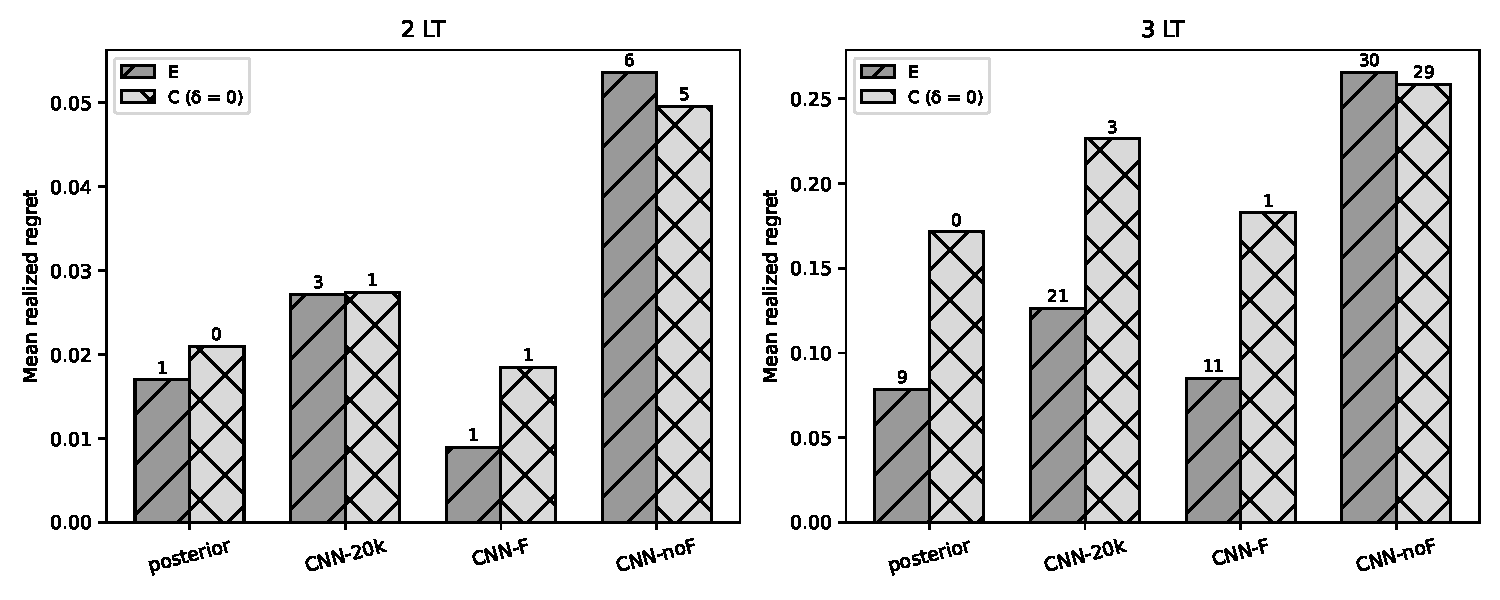
\includegraphics[width=\linewidth]{../figures/F17_decisions_paper.pdf}
\caption{Post hoc: mean realized regret of policies E (single hatching) and C with $\delta = 0$ (cross-hatching) for the posterior, CNN-20k and CNN-F at 2~LT (left) and 3~LT (right); the number above each bar is the count of instances harmed.}
\label{fig:xdecisions}
\end{figure}

\subsection{What procedures that inherit the forecast's horizon would answer}
\label{sec:procedures}
\paragraph{Forecast-horizon rules.} Take the last lead at which the forecast sign is confident for at least half the instances, which is 3~LT, answer every intervention-sign question up to that lead with the posterior's modal answer, and abstain beyond it. Through 3~LT the rule answers all 9600 intervention-sign questions and, in a post hoc tally, is right on 8965 (93.4\%). Where the posterior is confident (7116 questions) the two agree, and those answers are right 99.7\% of the time (19 wrong). The rest, 25.9\% of the questions in that range (27.6\% at 2~LT, 59.6\% at 3~LT), are answered without posterior confidence and are right 75.2\% of the time (77.6\% at 2~LT, 73.6\% at 3~LT). Beyond 3~LT the rule refuses every question, including those the posterior answers confidently (14.25\% of questions at 4~LT and 0.69\% at 6~LT). Post hoc, a per-instance version, which answers an instance's intervention questions at a lead whenever that instance's forecast sign is confident there, is right on 94.1\% of its answers through 3~LT; it answers without posterior confidence 23.7\% of intervention-sign questions at 2~LT and 37.4\% at 3~LT, and is right on 75.7\% and 73.0\% of those.

\paragraph{A perturbed-last-frame ensemble.} We form a 128-member ensemble by perturbing the last observed frame with the observation noise and using the forcing estimated from the observations by a one-dimensional fit. At 2~LT it is confident on 38.8\% of intervention signs, against the posterior's 72.4\%, and its confident observation-dependent answers are right 98.5\% of the time (lower bound 95.3\%). It is reliable but answers less; Cohen's $\kappa$ with the posterior's classifications is 0.48.

\paragraph{An ensemble smoother (development panel).} A randomized-maximum-likelihood ensemble smoother \citep{kitanidis1995quasilinear,oliver1996conditioning}, which is not an exact posterior sampler for a nonlinear model \citep{ba2022randomized}, was run as an independent cross-check on the development panel. It agrees with the posterior's intervention-sign classifications with $\kappa = 0.965$ at 2~LT and 0.934 at 3~LT, and gives the same confident shares to within two points.

%======================================================================
\section{Measuring for the decision}
\label{sec:measure}
If an intervention's effect has its own horizon, measurements chosen for the forecast need not be the ones that resolve it. In the first 60 confirmation instances (by index) in which the comparison between the two interventions with the lowest posterior-mean cost was not confident at 2~LT, we added four precise point measurements of the state at time zero, with noise one tenth of the observation noise. The sites were chosen by one of four rules: (Q) greedily reducing the posterior variance of the decision difference, as in ensemble-sensitivity targeting \citep{xie2013observing}; (F) the same rule for the unforced forecast; (V) largest posterior variance of the state, the family \citet{lorenz1998optimal} found best for forecast error; and (R) random sites. We then resampled the posterior (Table~\ref{tab:measure}). No arm produced a confident wrong answer. On the development panel, question-targeted measurement resolved 27 of 60 decisions against at most 13, with every McNemar $p < 0.001$. On the confirmation panel it resolved 15 against 10, 7 and 4. Against random sites it met the frozen 1\% level ($p = 0.004$); against spread-targeted sites it did not meet it ($p = 0.011$), and against forecast-targeted sites it did not reach it ($p = 0.0625$). The frozen criterion required a margin of 0.10, $p \le 0.01$ against all three, at least 20 confident answers with an exact one-sided 95\% accuracy lower bound of at least 0.80, and post-measurement truth coverage of at least 0.85. Arm Q resolved 15 confidently and correctly (lower bound 0.82, coverage 91.7\%), so the margin, the paired tests and the count all fell short, and the advantage did not confirm.

\begin{table}[t]
\centering
\small
\caption{Targeted measurement at 2~LT: instances (of 60) in which the decision question became confident and correct after four added measurements. $p$: exact one-sided McNemar test of arm Q against each arm.}
\label{tab:measure}
\begin{tabular}{lcccc}
\toprule
 & Q (decision) & F (forecast) & V (spread) & R (random) \\
\midrule
Confirmation & 15 & 10 ($p = 0.0625$) & 7 ($p = 0.011$) & 4 ($p = 0.004$) \\
Development  & 27 & 13 ($p = 2.6\times10^{-4}$) & 7 ($p = 1.8\times10^{-5}$) & 6 ($p = 4.8\times10^{-7}$) \\
\bottomrule
\end{tabular}
\end{table}

%======================================================================
\section{Discussion}
\label{sec:discussion}

\paragraph{Two signs, two functionals.} The forecast sign asks on which side of the climatological mean the posterior's window energies lie. The intervention sign asks whether the draws agree on the sign of a small difference that each computes along its own trajectory. Proposition~\ref{prop:small} shows that for small interventions this is a question about the tangent response, and that the near-perfect correlation of factual and counterfactual futures, which makes it tempting to expect the effect to outlast the forecast, is guaranteed by smallness and does not by itself determine the sign's confidence: in these results confidence falls as $c$ grows at fixed amplitude, but shrinking $a$ sends $c$ to zero without changing the limiting confidence. Shared uncertainty does help at first, and helps a great deal (the median $z_D$ is 3.6 times the median $z_F$ at lead 0). The budget shows where the draws' disagreement lies. The forcing change does work on the state directly, and to first order that part depends only on the unforced trajectory, which the posterior knows well. It also shifts the mean state (for a zero-mean pattern, only through the advection term's dependence on the state's short-range spatial covariance), and the unchanged forcing then does work on that shift. That indirect part depends on the tangent-linear dynamics along each draw's trajectory, and, post hoc and descriptively, beyond 1~LT it carries almost all of the draws' disagreement about the effect. Accurate marginal forecasts are not enough to answer an intervention question: what matters is the joint behaviour of the paired futures, and for the zero-mean patterns in particular the part of the response that runs through the flow's own nonlinearity.

\paragraph{Amplitude.} In the small-amplitude limit neither the posterior's confidence nor climatology's depends on how large the intervention is. The confirmation panel is close to that limit at 2~LT for amplitudes up to 2\% of the forcing. At 8\% the confident share rises and climatology starts to give some signs at longer leads, and the paired ordering weakens but holds. Linear response theory, including fluctuation--dissipation relations \citep{leith1975climate,majda2010high,marconi2008fluctuation}, describes the attractor-mean response at small amplitude; for one instance, what matters is the posterior distribution of the instance's own response, and its higher-order terms once the intervention is no longer small.

\paragraph{What a world model would need to report.} A world model used to choose actions is asked interventional questions, and its forecast skill against lead time does not say how far ahead those can be answered. At 3~LT the posterior-mean forecast in this system still has an anomaly correlation of 0.93, but the intervention sign is confident for 37\% of the seven non-uniform patterns' questions (post hoc). A rule that trusts interventional answers out to the forecast horizon is right on 93\% of its answers there, but on the quarter of questions the posterior withholds it is wrong one time in four, against about one in 375 of the posterior's confident answers over the same leads. The quantity to report is confidence per question, computed for the question being asked, from the joint distribution of the factual and counterfactual futures, and checked against realized outcomes. Our emulator results show why the check matters: two emulators with the same forecast skill and the same rate of confident answers differ in how often those answers are wrong (5.4\% against 0.8\%, averaged over instances); forecast skill does not reveal the difference, and scoring effect predictions against true effects, which a twin experiment supplies, does. That one of them passes matters as much as that one does not: the evaluation is one a learned model can meet. This echoes \citet{tan2026latent}, who find that what physical information a latent world model holds depends on its prediction target; here, what can be answered depends on the question. Goal-oriented experimental design \citep{zhong2026goaloriented,go2026goaldriven} and per-prediction observability \citep{kreutz2012likelihood} provide the machinery for asking it. In our decision analysis, requiring confidence before acting traded average regret for avoiding harm in these 200 instances; which side of that trade to take is a property of the application, not of the model. The development panel suggested that targeting measurements at the decision question helps; the confirmation panel did not confirm it.

\section{Limitations}
\begin{itemize}
\item This is a perfect-model twin: the declared law is the true law, and only the state and a uniform forcing are unknown. A two-scale model-error arm was planned and cut for compute. The posterior is a reference conditional on the declared model and prior.
\item Two costs (global and block window energy), one observation design (all sites, 0.84~LT, 2\% noise) and eight intervention patterns at three amplitudes were tested. The ordering may differ for other costs, sparser observations or longer windows. The forecast horizon is set by one sign question on the same cost; another forecast question would give another horizon.
\item Every analysis marked post hoc (the threshold sweep, censoring, indicator-precision and borderline readings; the seven-pattern, all-eight and per-pattern comparisons; confidence re-entry and last-confident endpoints; conventional forecast skill; the tangent response, energy budget and variance decomposition; the block observable; the confirmation-panel amplitudes; the full-range step-size check; the emulator comparisons; the decision analyses, including the cross-model decisions and the sizes of withheld effects; the worked instance; and the per-instance horizon rule) was added after the confirmation reading; their intervals carry no adjustment for that choice. The development-panel amplitude sweep has no realized-outcome scoring at the changed amplitudes.
\item The emulator comparison does not separate the forcing input, the training range of the forcing, noise-free training histories and training-set size. The paired-loss emulator (CNN-F-resp, Appendix~\ref{app:emulators}) used one untuned weight. Two further emulators from an earlier unpublished experiment of ours, CNN-20k fine-tuned on two-branch rollouts and, for one, also on paired differences, could not be evaluated because their checkpoints were not found.
\item Outside a twin or a repeatable matched-state experiment, an instance's effect sign is never observed. Randomized interventions across many instances can validate policy outcomes and mean effects, but the probability that an action helps a given instance depends on the joint distribution of its factual and counterfactual outcomes, which such data do not identify without further assumptions \citep{callaway2020bounds}. Here the known law supplies that coupling.
\item The ensemble-smoother cross-check ran on the development panel only. Truth coverage relies on Wilks' theorem and is approximate.
\end{itemize}

\section{Conclusion}
In this perfect-model Lorenz-96 setting we measured how confidence in an instance-specific intervention effect evolves relative to confidence in the factual forecast, checked those answers against the hidden truth, and located the physical response that carries the uncertainty. The posterior for one observed instance can say how far ahead each question about it can be answered, and the answer differs by question. Just after the observations the sign of a small intervention's effect is confident about as often as the forecast sign. Its observation-dependent confident share is lower than the forecast sign's at 2 and 3~LT (pre-registered); post hoc, its all-confident share is lower from 1.5 to 4~LT, and each of the seven patterns whose sign the observations must supply shows the same ordering at 2 and 3~LT. In the pre-registered paired comparison its confidence is lost first more often than not, despite factual and counterfactual futures that share almost all their uncertainty. That sharing is guaranteed when the intervention is small and does not settle the sign, which is decided by the instance's own response; post hoc, the draws disagree mainly about the part of that response that runs through the mean flow. In this setting the forecast horizon is not the intervention horizon, and a model used to act would need to report the second.

\section*{Reproducibility}
The frozen protocol, code, hashed per-case receipts, figures and a registry of every reported number, with a checker that regenerates it from the receipts, will be released in a public GitHub repository [URL to be added]. Every number in this paper is traceable to that registry or to the receipts it indexes.

\bibliographystyle{abbrvnat}
\bibliography{refs}

\appendix
\section{Additional emulator results}
\label{app:emulators}
CNN-F-resp adds to CNN-F's loss a paired loss on the difference between rollouts from one start under two actions, weighted so that the two losses start equal (4.11 GPU-hours). Trained at the weight fixed by that normalization rule, it is worse than CNN-F in state skill, cost error, confident-answer error and calibration: its state forecasts degrade (anomaly correlation 0.938), its window energies are biased low (mean $J_8$ error $-0.41$), 9.9\% of its confident intervention-sign answers are wrong, and its mean calibration is rejected (Table~\ref{tab:resp}). Acting on its predicted costs at 3~LT harms 30 of the 200 instances, and 9 when gated on its own confidence. On a fixed probe of training starts, the final model's weighted paired loss was 34 times its state loss (97\% of the objective): the weight that made the two losses equal at the start let the paired term dominate by the end. We did not tune that weight, and we do not read this as evidence against training on paired differences. A fourth model, with a head trained to predict window costs directly, is shown in Figure~\ref{fig:emulators_full} for completeness but is not interpretable here: the no-action option was absent from its training actions, so its no-action cost is an extrapolation.

\begin{table}[h]
\centering
\small
\caption{Post hoc: CNN-F-resp at 2~LT, in the format of Table~\ref{tab:emulators}.}
\label{tab:resp}
\footnotesize
\setlength{\tabcolsep}{4pt}
\begin{tabular}{lcccccc}
\toprule
Model & ACC / RMSE & $D$ error & confident $S$ & error [bounds] & overconfidence [99\%] & paired [99\%] \\
\midrule
CNN-F-resp & 0.938 / 0.248 & 0.141 & 72.1\% & 9.9\% [8.0, 13.5] & $+0.118$ [$0.052$, $0.184$] & $-0.384$ [$-0.524$, $-0.196$] \\
\bottomrule
\end{tabular}
\end{table}

\begin{figure}[h]
\centering
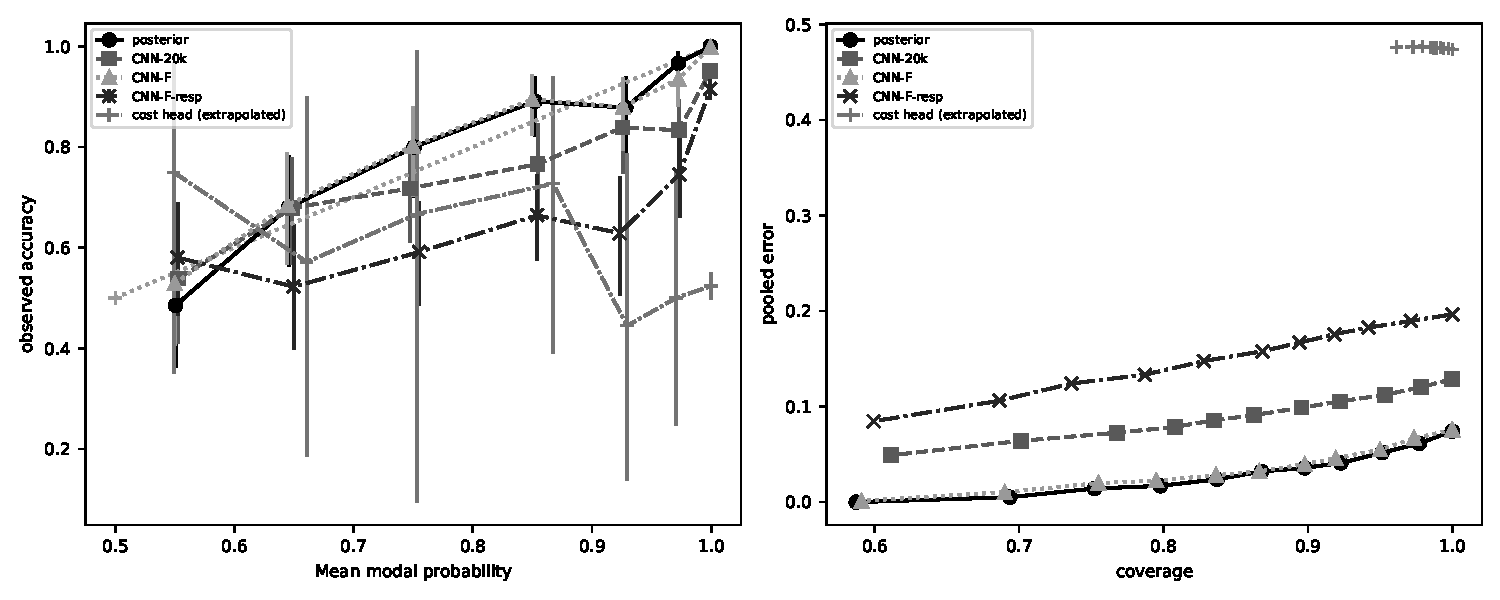
\includegraphics[width=\linewidth]{../figures/F13_reliability_paper.pdf}
\caption{Post hoc: as Figure~\ref{fig:emulators}, with all emulators. Posterior (solid, circles), CNN-20k (dashed, squares), CNN-F (dotted, triangles), CNN-F-resp (dash-dot, crosses) and the direct cost head (plus signs; not interpretable, see text). The dotted diagonal marks perfect reliability.}
\label{fig:emulators_full}
\end{figure}

\section{Confident shares by question type}
\label{app:shares}
\begin{figure}[h]
\centering
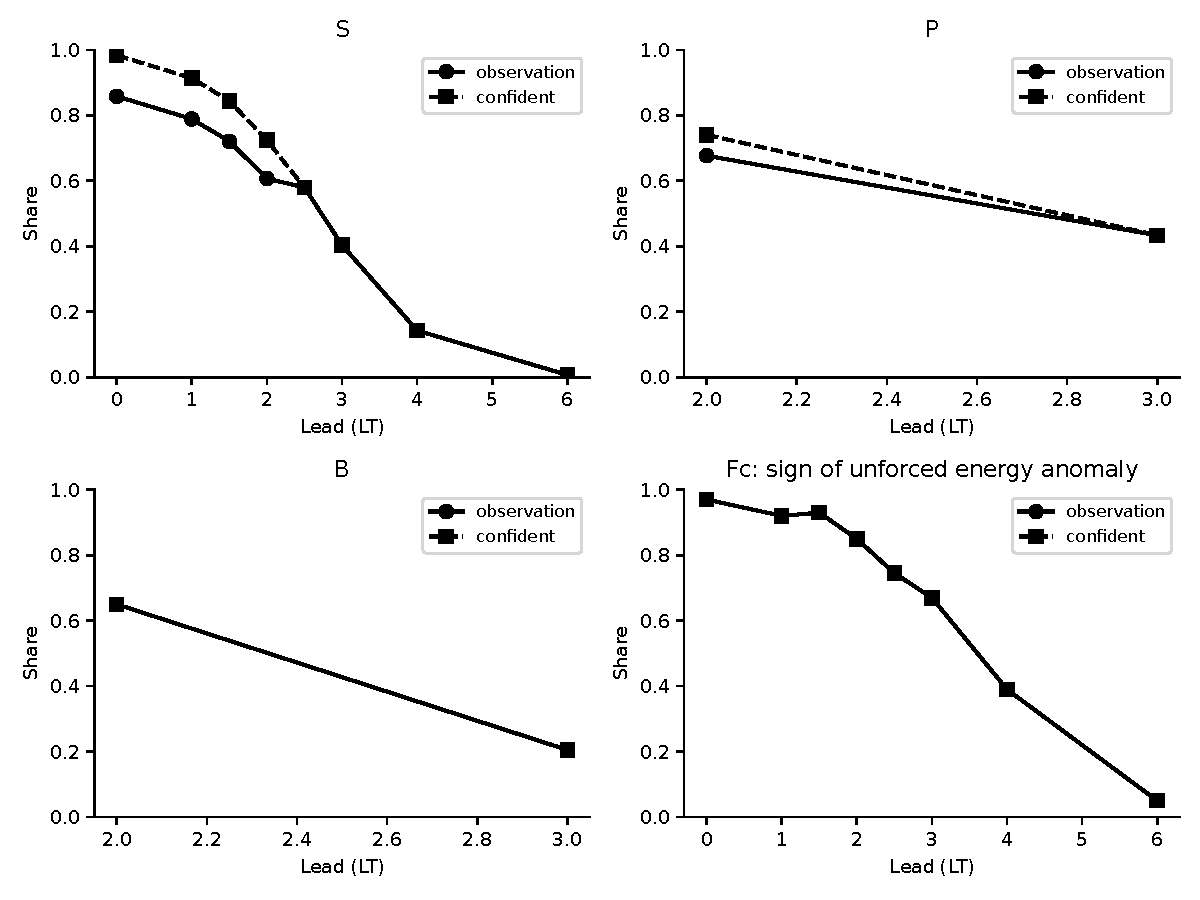
\includegraphics[width=0.92\linewidth]{../figures/F2_confidence.pdf}
\caption{Share of questions answered confidently against lead, confirmation panel. Solid circles: observation-confident; dashed squares: all confident. Panels: intervention sign $S$, pairwise order $P$, best action $B$, and the forecast sign $F_c$ (the sign of the unforced window-energy anomaly). $P$ and $B$ are reported at 2 and 3~LT only.}
\label{fig:confidence}
\end{figure}

\end{document}
